\documentclass[dvipsnames, svgnames,a4paper,11pt]{article}
\usepackage{todonotes}
% ----------------------------------------------------- 
%	加边框的命令
%	参考:https://tex.stackexchange.com/questions/531559/how-to-add-the-page-border-for-first-two-pages-in-latex
\usepackage{tikz}
\usetikzlibrary{calc}
\usepackage{eso-pic}
\AddToShipoutPictureBG{%
\begin{tikzpicture}[overlay,remember picture]
\draw[line width=0.6pt] % 边框粗细
    ($ (current page.north west) + (0.6cm,-0.6cm) $)
    rectangle
    ($ (current page.south east) + (-0.6cm,0.6cm) $); % 边框位置
\end{tikzpicture}}


\usepackage{xcolor}
\definecolor{c1}{HTML}{2752C9} % 目录颜色
\definecolor{c2}{RGB}{190,20,83} % 引用颜色

\usepackage{ctex}
\usepackage[top=28mm,bottom=28mm,left=15mm,right=15mm]{geometry} % 调整边距
\usepackage{hyperref} 
\hypersetup{
	colorlinks,
	linktoc = section, % 给目录加的超链接位置,选项有 section, page, all
	linkcolor = c1, % linkcolor 目录颜色
	citecolor = c1  % citecolor 引用颜色
}
\usepackage{amsmath,enumerate,multirow,float}
\usepackage{tabularx}
\usepackage{tabu}
\usepackage{subfig}
\usepackage{fancyhdr}
\usepackage{graphicx}
\usepackage{wrapfig}  
\usepackage{physics}
\usepackage{appendix}
\usepackage{amsfonts}
\usepackage{annotate-equations} % 公式标注
\usepackage{pgfplots} % pgf 绘图


% ---------------------------------------------------------------------
%	定义了两类colorbox
\usepackage{tcolorbox}
\tcbuselibrary{skins,breakable}
\newtcolorbox{tbox}[2][]{
    colframe=black!70!,
    breakable,
    enhanced,
    boxrule =0.5pt,
    title = {#2},
    fonttitle = \large\bfseries,
    drop fuzzy shadow,
    #1
}
\newtcolorbox[auto counter,number within=section]{question}[1][]{
  top=2pt,bottom=2pt,arc=1mm,
  boxrule=0.5pt,
  breakable,
  enhanced, % 跨页后不会显示下边框
  coltitle=c1!80!gray,
  colframe=c1,
  colback=c1!3!white,
  drop fuzzy shadow,
  title={思考题~\thetcbcounter:\quad},
  fonttitle=\bfseries,
  attach title to upper,
  #1
}

% ---------------------------------------------------------------------
%	利用 cleveref 改变引用格式,\cref 是引用命令
\usepackage{cleveref}
\crefformat{figure}{#2{\textcolor{c2}{图 #1}}#3} % 图片的引用格式
\crefformat{equation}{#2{(\textcolor{c2}{#1})}#3} % 公式的引用格式
\crefformat{table}{#2{\textcolor{c2}{表 #1}}#3} % 表格的引用格式


% ---------------------------------------------------------------------
%	页眉页脚设置
\fancypagestyle{plain}{\pagestyle{fancy}}
\pagestyle{fancy}
\lhead{\kaishu 中山大学物理与天文学院近代物理实验\uppercase\expandafter{\romannumeral1}} % 左边页眉,学院 + 课程
\rhead{\kaishu 材料真空兼容测试和等离子特性研究 实验报告} % 右边页眉,实验报告标题
\cfoot{\thepage} % 页脚,中间添加页码
\setlength{\headheight}{13.6pt}

% ---------------------------------------------------------------------
%	对目录、章节标题的设置
\renewcommand{\contentsname}{\centerline{\huge 目录}}
\usepackage{titlesec}
\usepackage{titletoc}
% \titleformat{章节}[形状]{格式}{标题序号}{序号与标题间距}{标题前命令}[标题后命令]
\titleformat{\section}{\centering\LARGE}{}{1em}{}
\newcommand{\nsection}[3]{%
    \section{#1 #2 \hspace{11pt} \textbf{#3}}%
}

% ---------------------------------------------------------------------
%   listing代码环境设置
\usepackage{listings}
\lstloadlanguages{python}
\lstdefinestyle{pythonstyle}{
backgroundcolor=\color{gray!5},
language=python,
frameround=tftt,
frame=shadowbox, 
keepspaces=true,
breaklines,
columns=spaceflexible,                   
basicstyle=\ttfamily\small, % 基本文本设置,字体为 teletype,大小为 small
keywordstyle=[1]\color{c1}\bfseries, 
keywordstyle=[2]\color{Red!70!black},   
stringstyle=\color{Purple},       
showstringspaces=false,
commentstyle=\ttfamily\scriptsize\color{green!40!black}, % 注释文本设置,字体为 teletype,大小为 scriptsize
tabsize=2,
morekeywords={as},
morekeywords=[2]{np, plt, sp},
numbers=left, % 代码行数,位置在左
numberstyle=\it\tiny\color{gray}, % 代码行数的数字字体设置
stepnumber=1,
rulesepcolor=\color{gray!30!white}
}


% ---------------------------------------------------------------------
%	将表格封装起来
\newcommand{\scoresTable}[8]{
    \begin{table}
        \renewcommand\arraystretch{1.7}
        \begin{tabularx}{\textwidth}{
                |X|X|X|X
                |X|X|X|X|}
            \hline
            \multicolumn{2}{|c|}{预习报告} & \multicolumn{2}{|c|}{实验记录} & \multicolumn{2}{|c|}{分析讨论} & \multicolumn{2}{|c|}{总成绩} \\
            \hline
            \centering#1&\centering#2 &\centering#3 &\centering#4 &\centering#5 &\centering#6 &\centering#7 &{\centering#8} \\
            \hline
        \end{tabularx}
    \end{table}
}
\newcommand{\infoTable}[6]{
    \begin{table}
        \renewcommand\arraystretch{1.7}
        \begin{tabularx}{\textwidth}{|X|X|X|X|}
        \hline
        专业:& #1 &年级:& #2\\
        \hline
        姓名:& #3   & 学号:&#4\\
        \hline
        实验时间:&#5 & 教师签名:&#6 \\
        \hline
        \end{tabularx}
    \end{table}
}

% ---------------------------------------------------------------------
%	其他设置
\def\degree{${}^{\circ}$} % 角度
\graphicspath{{./images/}} % 插入图片的相对路径
\allowdisplaybreaks[4]  %允许公式跨页

\usetikzlibrary{patterns,decorations.markings,arrows.meta,bending} % TikZ 包的拓展 % 导入模板的相关设置
\usepackage{lipsum}
\usepackage{amsmath}
\usepackage{array}

\usepackage{tabularx}
\usepackage{graphicx}


\begin{document}

\scoresTable{}{}{}{}{}{}{}{}

% \infoTable{专业}{年级}{姓名}{学号}{实验时间}{教师签名}
\infoTable{物理学}{2022级}{丁侯凯}{22344009}{2024.9.18}{}

\begin{center}
	\LARGE D1 \quad 锁相放大器与弱信号测量
\end{center}

\textbf{【实验报告注意事项】}
\begin{enumerate}
	\item 实验报告由三部分组成:
	\begin{enumerate}
		\item 预习报告:(提前一周)认真研读\underline{\textbf{实验讲义}},弄清实验原理;实验所需的仪器设备、用具及其使用(强烈建议到实验室预习),完成课前预习思考题;了解实验需要测量的物理量,并根据要求提前准备实验记录表格(第一循环实验已由教师提供模板,可以打印)。预习成绩低于10分(共20分)者不能做实验。
	    \item 实验记录:认真、客观记录实验条件、实验过程中的现象以及数据。实验记录请用珠笔或者钢笔书写并签名(\textcolor{red}{\textbf{用铅笔记录的被认为无效}})。\textcolor{red}{\textbf{保持原始记录,包括写错删除部分,如因误记需要修改记录,必须按规范修改。}}(不得输入电脑打印,但可扫描手记后打印扫描件);离开前请实验教师检查记录并签名。
	    \item 分析讨论:处理实验原始数据(学习仪器使用类型的实验除外),对数据的可靠性和合理性进行分析;按规范呈现数据和结果(图、表),包括数据、图表按顺序编号及其引用;分析物理现象(含回答实验思考题,写出问题思考过程,必要时按规范引用数据);最后得出结论。
	\end{enumerate}
	\textbf{实验报告就是将预习报告、实验记录、和数据处理与分析合起来,加上本页封面。}
	\item 每次完成实验后的一周内交\textbf{实验报告}(特殊情况不能超过两周)。
	\item 除实验记录外,实验报告其他部分建议双面打印。
\end{enumerate}


\clearpage
\tableofcontents
\clearpage

\setcounter{section}{0}
\nsection{D1}{锁相放大器与弱信号测量}{预习报告}
	
\subsection{实验目的}
\begin{enumerate}
	\item 了解锁相放大器工作原理和特点,理解信号、噪声、信噪比等概念。
	\item  掌握锁相放大器基本参数含义及锁相放大器的基本操作,学会合理选择或调节参数(频率、相位、灵敏度、时间常数、陡降);复习示波器的使用。
	\item 掌握用锁相放大器检测弱信号方法,通过与示波器比较其检测能力了解其技术优势。
\end{enumerate}

\subsection{仪器用具}
\begin{table}[htbp]
	\centering
	\renewcommand\arraystretch{1.6}
	% \setlength{\tabcolsep}{10mm}
	\begin{tabular}{p{0.05\textwidth}|p{0.20\textwidth}|p{0.05\textwidth}|p{0.5\textwidth}}
	\hline
	编号& 仪器用具名称 & 数量 &  主要参数(型号,测量范围,测量精度等) \\
	\hline
	1&锁相放大器 &1 & OE1022(系列)\\
	2&配套教学实验箱 &1 & \\
	3&示波器 &1 & RIGOL DS2202A\\
	4&信号发生器 &1 &RIGOL DG4162 \\
	5&BNC-BNC 信号线 &1 &若干 \\

	\hline
\end{tabular}
\end{table}

\subsection{原理概述}
		% \begin{wrapfigure}{l}{0cm} % l 表示靠文字内容的左侧,0cm 表示环境横向长度
		% 	\centering
		% 	
\includegraphics[width=0.3\textwidth]{example.png}
		% 	\caption{环绕图片示例}
		% \end{wrapfigure}
		% \textcolor{red}{参考文献示例},参考\cite{test1,test2}。
		\subsubsection{锁相放大器(Phase-Locked Amplifier, LIA)}

		锁相放大器是从强噪声背景中提取出微弱的特定频率信号。它通过与一个已知频率的参考信号进行相位锁定,从而筛选出与参考频率同步的信号分量。LIA可以极大提高信号的信噪比,使其能够检测出极其微弱的信号。

		\subsubsection{工作原理}
			锁相放大器的基本原理是相敏检测,设输入信号 
			\( V_{\text{in}}(t) \) 通常为目标信号与噪声的叠加:
			\[
			V_{\text{in}}(t) = V_{\text{signal}}(t) + V_{\text{noise}}(t)
			\]
			其中 \( V_{\text{signal}}(t) \) 是待测信号,\( V_{\text{noise}}(t) \) 是背景噪声。

			LIA通过一个混频器将输入信号与参考信号 \( V_{\text{ref}}(t) \) 相乘。参考信号通常为正弦或余弦波:
			\[
			V_{\text{ref}}(t) = A_{\text{ref}} \cos(\omega_{\text{ref}} t + \phi_{\text{ref}})
			\]
			其中,\( \omega_{\text{ref}} \) 为参考信号的角频率,\( \phi_{\text{ref}} \) 为参考信号的相位。再将输入信号 \( V_{\text{in}}(t) \) 与参考信号 \( V_{\text{ref}}(t) \) 相乘:
			\[
			V_{\text{mixed}}(t) = V_{\text{in}}(t) \times V_{\text{ref}}(t)
			\]
			此时产生两个分量:一个是低频分量,与参考信号的相位差有关;另一个是高频分量,而高频分量则可以通过滤波去除。
			
			最后LIA通过低通滤波器去除高频分量,保留低频分量,即与参考信号相同频率、相位相关的部分。此时的输出信号与待测信号的相位差成比例:
			\[
			V_{\text{out}} \propto \cos(\phi_{\text{signal}} - \phi_{\text{ref}})
			\]
			当待测信号与参考信号同步时,输出信号达到最大值。

		\subsubsection{公式推导}

		分别假设输入信号$V_{\text{in}}(t) $、参考信号$V_{\text{ref}}(t) $、混频器输出信号$V_{\text{mixed}}(t)$
		\[
		V_{\text{in}}(t) = A_{\text{signal}} \cos(\omega_{\text{signal}} t + \phi_{\text{signal}})
		\]
		其中,\( A_{\text{signal}} \) 是信号的幅值,\( \omega_{\text{signal}} \) 是信号的角频率,\( \phi_{\text{signal}} \) 是信号的相位。

		\[
		V_{\text{ref}}(t) = A_{\text{ref}} \cos(\omega_{\text{ref}} t + \phi_{\text{ref}})
		\]
		其中,\( A_{\text{ref}} \) 是参考信号的幅值,\( \omega_{\text{ref}} \) 是参考信号的角频率,\( \phi_{\text{ref}} \) 是参考信号的相位。

		将输入信号和参考信号相乘:
		\[
		V_{\text{mixed}}(t) = A_{\text{signal}} A_{\text{ref}} \cos(\omega_{\text{signal}} t + \phi_{\text{signal}}) \cos(\omega_{\text{ref}} t + \phi_{\text{ref}})
		\]
		
		再使用三角函数的乘积公式,可以将其展开为:
		\[
		V_{\text{mixed}}(t) = \frac{A_{\text{signal}} A_{\text{ref}}}{2} \left[ \cos((\omega_{\text{signal}} - \omega_{\text{ref}}) t + (\phi_{\text{signal}} - \phi_{\text{ref}})) + \cos((\omega_{\text{signal}} + \omega_{\text{ref}}) t + (\phi_{\text{signal}} + \phi_{\text{ref}})) \right]
		\]
		其中,低频成分 \( (\omega_{\text{signal}} - \omega_{\text{ref}}) \) 是待测信号与参考信号之间的相位差。

		通过低通滤波器后,保留的仅是低频成分:
		\[
		V_{\text{out}} = \frac{A_{\text{signal}} A_{\text{ref}}}{2} \cos(\phi_{\text{signal}} - \phi_{\text{ref}})
		\]
		这个输出信号与待测信号的幅值 \( A_{\text{signal}} \) 和相位差 \( \phi_{\text{signal}} - \phi_{\text{ref}} \) 成正比。


\subsection{实验安全注意事项}
\begin{enumerate}
	\item OE1022锁相放大器输入端不能接入强信号,接入信号需限定在1V以下。
	\item OE4201 压控电流源的电流输出不能直接接入OE1022锁相放大器的输入端。
\end{enumerate}

\clearpage
\subsection{现场预习报告思考题}
	\begin{question}
		如何用锁相放大器检测到待测的直流信号或慢变信号(图1中的v(t))? 
	\end{question}

		
	\begin{figure}[htbp]
		\centering
		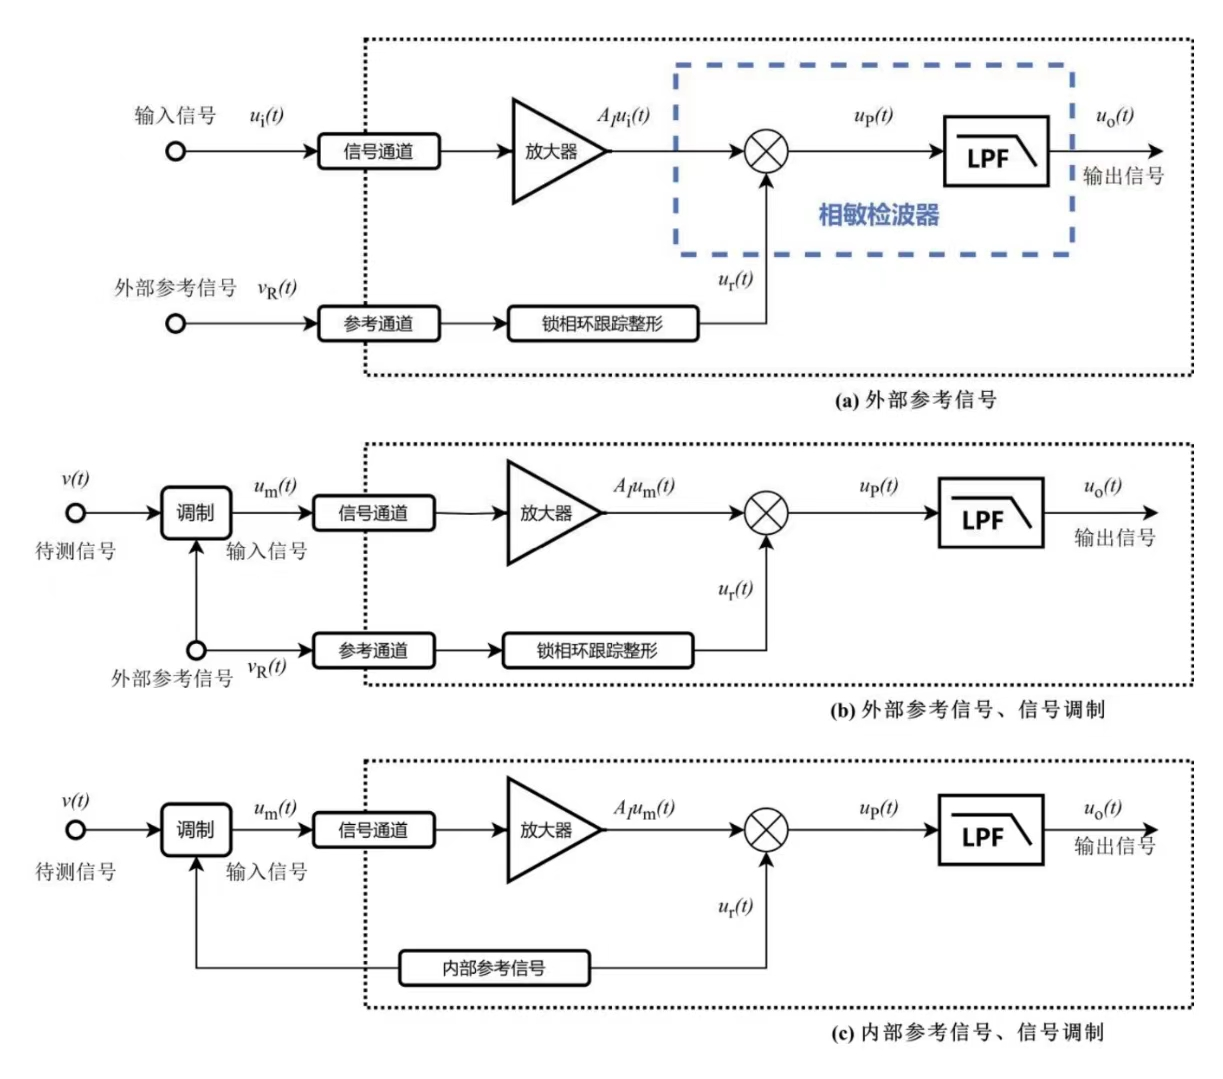
\includegraphics[width=0.75\textwidth]{锁相放大器流程图.jpg}
		\caption{锁相放大器流程图}
		\label{fig:锁相放大器流程图}
	\end{figure}
	对于直流信号或者慢变信号而言,输入的信号应该是非三角函数信号,此时需要按照流程图
	设调制前的信号包括待测信号与噪声:
	\begin{equation}
	v(t) = s(t) +n(t)
	\label{eq:1}
	\end{equation}
	经过$sin(\omega t + \theta)$调制后:$u_m(t) = v(t)sin(\omega _m t +\theta)$,此时的输入信号依旧十分微弱,经过前置放大器的放大$A_I$倍后,得到:
	$$
	u_a(t) = A_Is(t)	sin(\omega _m t +\theta)+A_I n(t)
	$$
	最后根据解调就可以得到从噪声中分离出来的信号。需要用乘法器将放大后的信号$u_a(t)$与参考信号$u_r(t)=sin(\omega _rt)$相乘:


	\begin{align}
		u_{px}(t) &= u_r(t)u_a(t) \nonumber \\
				  &= A_I[s(t)\sin(\omega_m t + \theta)\sin(\omega_r t) + n(t)\sin(\omega_r t)] \nonumber \\
				  &= A_I { \frac{s(t)}{2} \left[ \cos((\omega_m - \omega_r)t + \theta) - \cos((\omega_m + \omega_r)t + \theta) \right] + n(t)\sin(\omega_r t) } \label{eq:2}
	\end{align}
	由于调制信号使用参考信号通过某种物理机制触发或者用参考信号本身,参考信号与调制信号频率相同$\omega _m=\omega_r$、相位差$\theta$确定,因此通过理想低通滤波器滤去高频分量后,滤波器的输出信号为:
	\begin{align}
		u_{ox}(t)=A_I [ \frac{1}{2} s(t) cos\theta +n_x(t)] \label{eq:3}
	\end{align}
	其中$n_x(t)$为未被滤去的,且与参考信号频率相同的同频噪声。


		



	\begin{question}
	 噪声有哪些类型?一般测量对象本身的噪声是哪来的?它有什么特征?
	\end{question}
	1.噪声的类型

	1)热噪声

	由导体内部电子的热运动引起,随温度升高而增大,与电阻值成正比。任何电阻元件在温度不为绝对零度时都会产生热噪声。这种噪声存在于导体、电阻、电源和接收器等所有电路元件中。它是频率无关的,因此是一种白噪声,功率谱在各个频率上均匀分布。
	
	2)1/f 噪声
	
	也称为低频噪声,常见于电子器件中,尤其在低频段表现明显,随频率增加而衰减。其特点是频谱密度与频率成反比,广泛存在于半导体器件、导体和部分化学反应中。
	
	3)环境噪声

	包括来自电源线、无线电波、灯具、变压器等的电磁干扰,常表现为特定频率,如50/60Hz的工频噪声。

	4)相位噪声

	是频率或相位抖动引起的噪声,常见于振荡器、时钟电路等电子设备中,会影响信号的频率稳定性。

	2.测量对象噪声的特征

	1)白噪声特征

	在频域中,白噪声的功率谱密度是平坦的,它的功率在所有频率上均匀分布。热噪声是白噪声的典型例子。

	2)低频噪声特征(1/f噪声)

	测量中常遇到1/f噪声,其功率谱密度随频率增加而下降。这种噪声在低频时显著,通常是电阻、电流、电压测量中的主要噪声来源。

	3)非线性噪声

	有些噪声源(如散粒噪声)随测量信号的非线性关系变化,它们的功率与电流、温度或其它量度成非线性关系。


	\begin{question}
	是否可以用RIGOL DG4162信号发生器产生白噪声取代教学实验箱产生的白噪声?如何将它与信号混合? 
	\end{question}
	可以使用RIGOL DG4162 信号发生器产生白噪声来取代教学实验箱中的白噪声。该信号发生器支持多种波形输出,包括 白噪声 和 伪随机噪声,因此能够很好地模拟噪声信号,作为教学实验的一部分。

	与信号混合的方法过程:
	
	1)设置白噪声
	\begin{enumerate}
		\item 打开信号发生器:	进入波形菜单,并选择 Noise选项:白噪声是一种频谱均匀分布的噪声,在 DG4162 的噪声模式下可以直接产生。
		\item 通过菜单选项,调整噪声幅度 和 带宽,以生成适当的噪声信号。白噪声的幅度和频率带宽应根据实验的需求进行设置。
	\end{enumerate}
    
	2) 将噪声与信号混合

	方法一:使用外部电路进行混合

	使用信号发生器输出的噪声信号和其他信号,通过一个简单的电阻加法器电路(电压叠加电路)进行混合。该电路由电阻构成,两个信号的电压通过电阻叠加,实现信号和噪声的混合。
	\begin{enumerate}
		\item  将 信号 和 噪声 信号的输出分别连接到电阻加法器的输入端。
		\item 将加法器的输出连接到测量设备(例如示波器或实验箱的输入端)。
		\item 通过调节信号的幅度和噪声的强度,调整信噪比。
	\end{enumerate}
    
	方法二:使用RIGOL DG4162的内置功能

	RIGOL DG4162 也支持 双通道输出,即可以从一个通道输出信号,从另一个通道输出噪声。可以通过信号发生器的外部触发功能,将两个通道的信号合成,或者在后续的电路中叠加这两个通道的信号。
	\begin{enumerate}
		\item 在 通道 1 设置输出信号(例如正弦波)。
		\item 	在 通道 2 设置输出白噪声。
		\item 将两个通道的输出同时连接到一个加法电路或混合设备(如示波器的两个输入端,或外部的混合器),这样可以直接在同一测量系统中获取混合信号

	\end{enumerate}


	\begin{question}
	复习用示波器测量信号的实验步骤,学习用数字示波器中的带通滤波器过滤噪声的操作。 
	\end{question}

1.设置示波器:

   打开示波器,并确保通道和探头连接正确。探头应接到测量信号的信号源端,探头接地应接到信号源的地端。确认探头的衰减设置与示波器通道设置一致。

2. 调整示波器时基和电压范围:

  设置示波器的时间基,根据信号的频率范围调整,使信号可以在屏幕上显示出来。
  调整垂直刻度(电压范围),使信号的振幅显示得较为清晰。

3. 触发设置:

  设置触发电平,选择一个适当的触发点,以稳定地捕获信号。
 选择触发模式(如上升沿、下降沿等),确保信号在屏幕上稳定显示。

4. 观察和分析信号:

   观察信号的波形,调整垂直和水平控制,使波形显示更为清晰。
   使用示波器的测量工具,可以直接测量信号的频率、周期、振幅等。

5. 保存或记录数据:
   使用示波器的存储功能,可以保存波形图供后续分析。

   \vspace{1cm}


使用数字示波器中的带通滤波器过滤噪声:现代数字示波器通常带有带通滤波器功能,可以过滤特定频段的噪声,保留目标信号。

1. 找到滤波器选项:
   
在示波器的菜单中查找滤波器设置(通常在波形处理或信号处理菜单下)。
  选择带通滤波器(Band-pass Filter) 选项。

2. 设定带通滤波器的上下限频率:

   输入带通滤波器的下限频率和上限频率,以设定需要通过的信号频段。例如,如果信号频率为1kHz,设置带通滤波器的范围在900Hz到1100Hz之间,其他频率的噪声会被滤除。

3. 观察信号变化:
   
 应用滤波器后,观察屏幕上信号波形的变化。噪声被过滤后,信号应更加平滑。

4. 保存或导出滤波后的波形:
  
 经过滤波处理的信号可以用来进行更精准的测量。示波器通常支持导出数据和波形图,可以保存以供进一步分析。

 \vspace{1cm}
 实验注意事项:

  确保探头的接地和信号源的接地正确连接,避免引入额外的噪声。
 调整滤波器的频率范围时,需要基于目标信号的频率特性,以避免削弱有用信号。



\clearpage
\begin{table}
	\renewcommand\arraystretch{1.7}
	\centering
	\begin{tabularx}{\textwidth}{|X|X|X|X|}
	\hline
	专业:& 物理学 &年级:& 2019级 \\
	\hline
	姓名: & 丁侯凯& 学号:&22344009\\
	\hline
	室温:&24℃ & 实验地点: & A102\\
	\hline
	学生签名:& 
\includegraphics[width=2cm]{签名.jpg}      & 评分: &\\
	\hline
	实验时间:&2024.9.18 & 教师签名:&\\
	\hline
	\end{tabularx}
\end{table}

\nsection{D1}{锁相放大器与弱信号测量}{实验记录}
\subsection{实验内容和步骤}
	\subsubsection{用示波器观察内部信号输出(与参考信号同频同相}
		\begin{enumerate}
		\item 用OE1022的内部振荡器SINE OUT ,输出正弦信号,产生一个幅值为80m$V_{rms}$、频率约为1kHz的正弦波。
		\item 用示波器观察和记录波形及信号参数。记录如图\ref{fig:示波器正弦波}。
		\item 注意用三通分信号至示波器时,需要在示波器输入通道设置中选择输入阻抗为1MΩ,防止信号源的电压输出因为过大的电流损耗而被衰减。
		\end{enumerate}

		\begin{figure}[htbp]
			\centering
			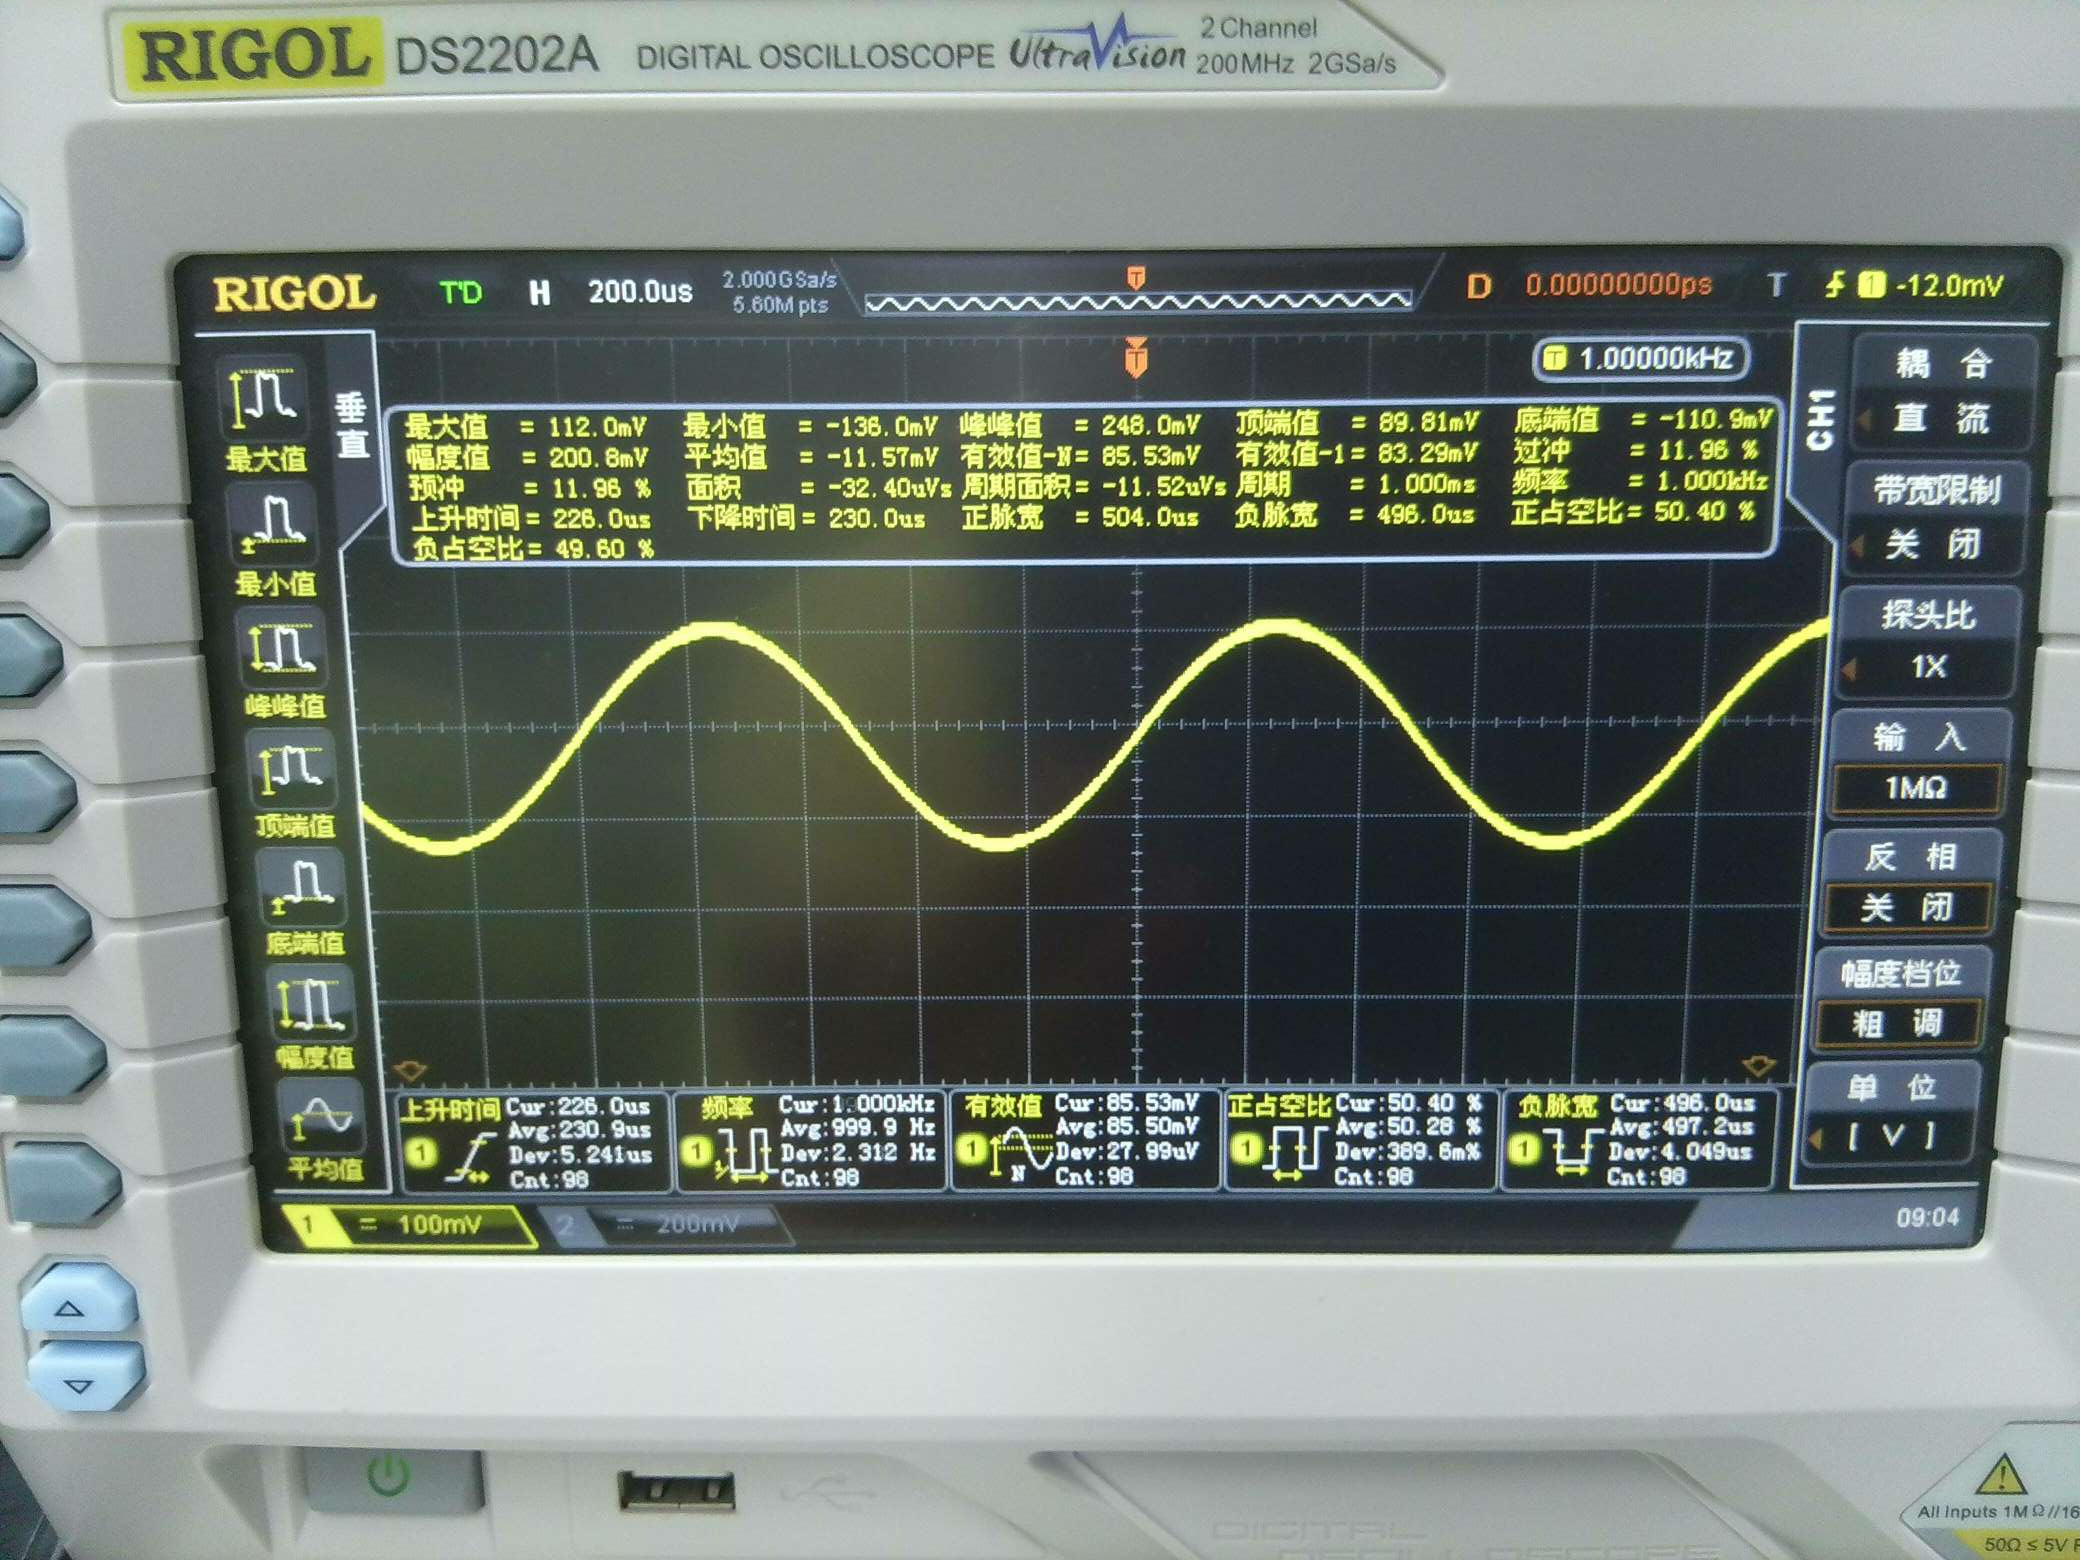
\includegraphics[width=0.75\textwidth]{示波器正弦波.png}
			\caption{用示波器观察内部信号输出为正弦波}
			\label{fig:示波器正弦波}
		\end{figure}



	\subsubsection{测量信号R、$\theta$、X以及Y值,并验证他们之间的关系}
		\begin{enumerate}
		\item 使用BNC-BNC信号线连接OE1022的SINE OUT输出接口与SIGNAL IN的A|I接口,观察检测栏的Overload是否提示溢出。若输入溢出,则显示Overload:INPUT NONE;若放大溢出,则显示Overload:NONE GAIN;若同时溢出,则显示Overload:INPUT GAIN。
		\item 实验中保证数字信号发生器输出赋值为80m$V_{rms}$的正弦波不会发生溢出。若有前级溢出时应立即减小数字信号发生器输出幅值,若有放大溢出应立即调节量程灵敏度(sensitivity)值。
		\item 面板GAIN/TC按键进入子菜单,调节量程灵敏度值。
		\item 选中Sensitivity功能,通过旋转旋钮调节Sensitivity值,使测量信号值尽量满偏而又不超量程,即简单测出了从内置函数信号发生器输出的正弦波幅值大小以及相位。 
		\item 键进入子菜单可以挑选实时显示R、$\theta$、X、Y值。
		\end{enumerate}

	\subsubsection{相敏检波器工作原理——乘法器}
		\begin{enumerate}
			\item 使用信号发生器输出一个幅值约为50m$V_{rms}$、频率约为1kHz的正弦波,并输入进OE1022锁相放大器中。
			\item 将滤波器带宽调至最大,使TC=10us、Slope=6dB/oct,此时锁相放大器的输出可以等效于乘法器输出。
			\item 将锁相放大器模拟输出(Fast channel out)连接到示波器的输入进行观察。注意信号是否超量程,调节信号幅值或量程灵敏度(sensitivity)使之在合适量程以内。
		\end{enumerate}
	
	\subsubsection{相敏检波器工作原理——乘法器+低通滤波器}
		\begin{enumerate}
			\item 设置滤波器时间常数和陡降,如表\ref{tab:1}所示)。
			\item 通过示波器同时分别观察和记录锁相放大器的输入信号波形、乘法器输出(CHANNEL OUTPUT)的R、X、Y波形,以及锁相放大器的R、X、Y读数。
			\item 选择并保持某个时间常数,使得TC小于输入信号周期,改变滤波器的陡降(6、12、18、24dB/oct),观察并记录示波器波形的变化。实验记录如表 \ref{tab:2}  所示。
		\end{enumerate}

		\begin{table}[ht]
			\centering
			\begin{tabularx}{\textwidth}{|c|X|X|X|}
				\hline
				% 第一行表头
				时间常数 & R波形  & X波形  & Y波形 \\
				\hline
				% 数据行 1
				10us & 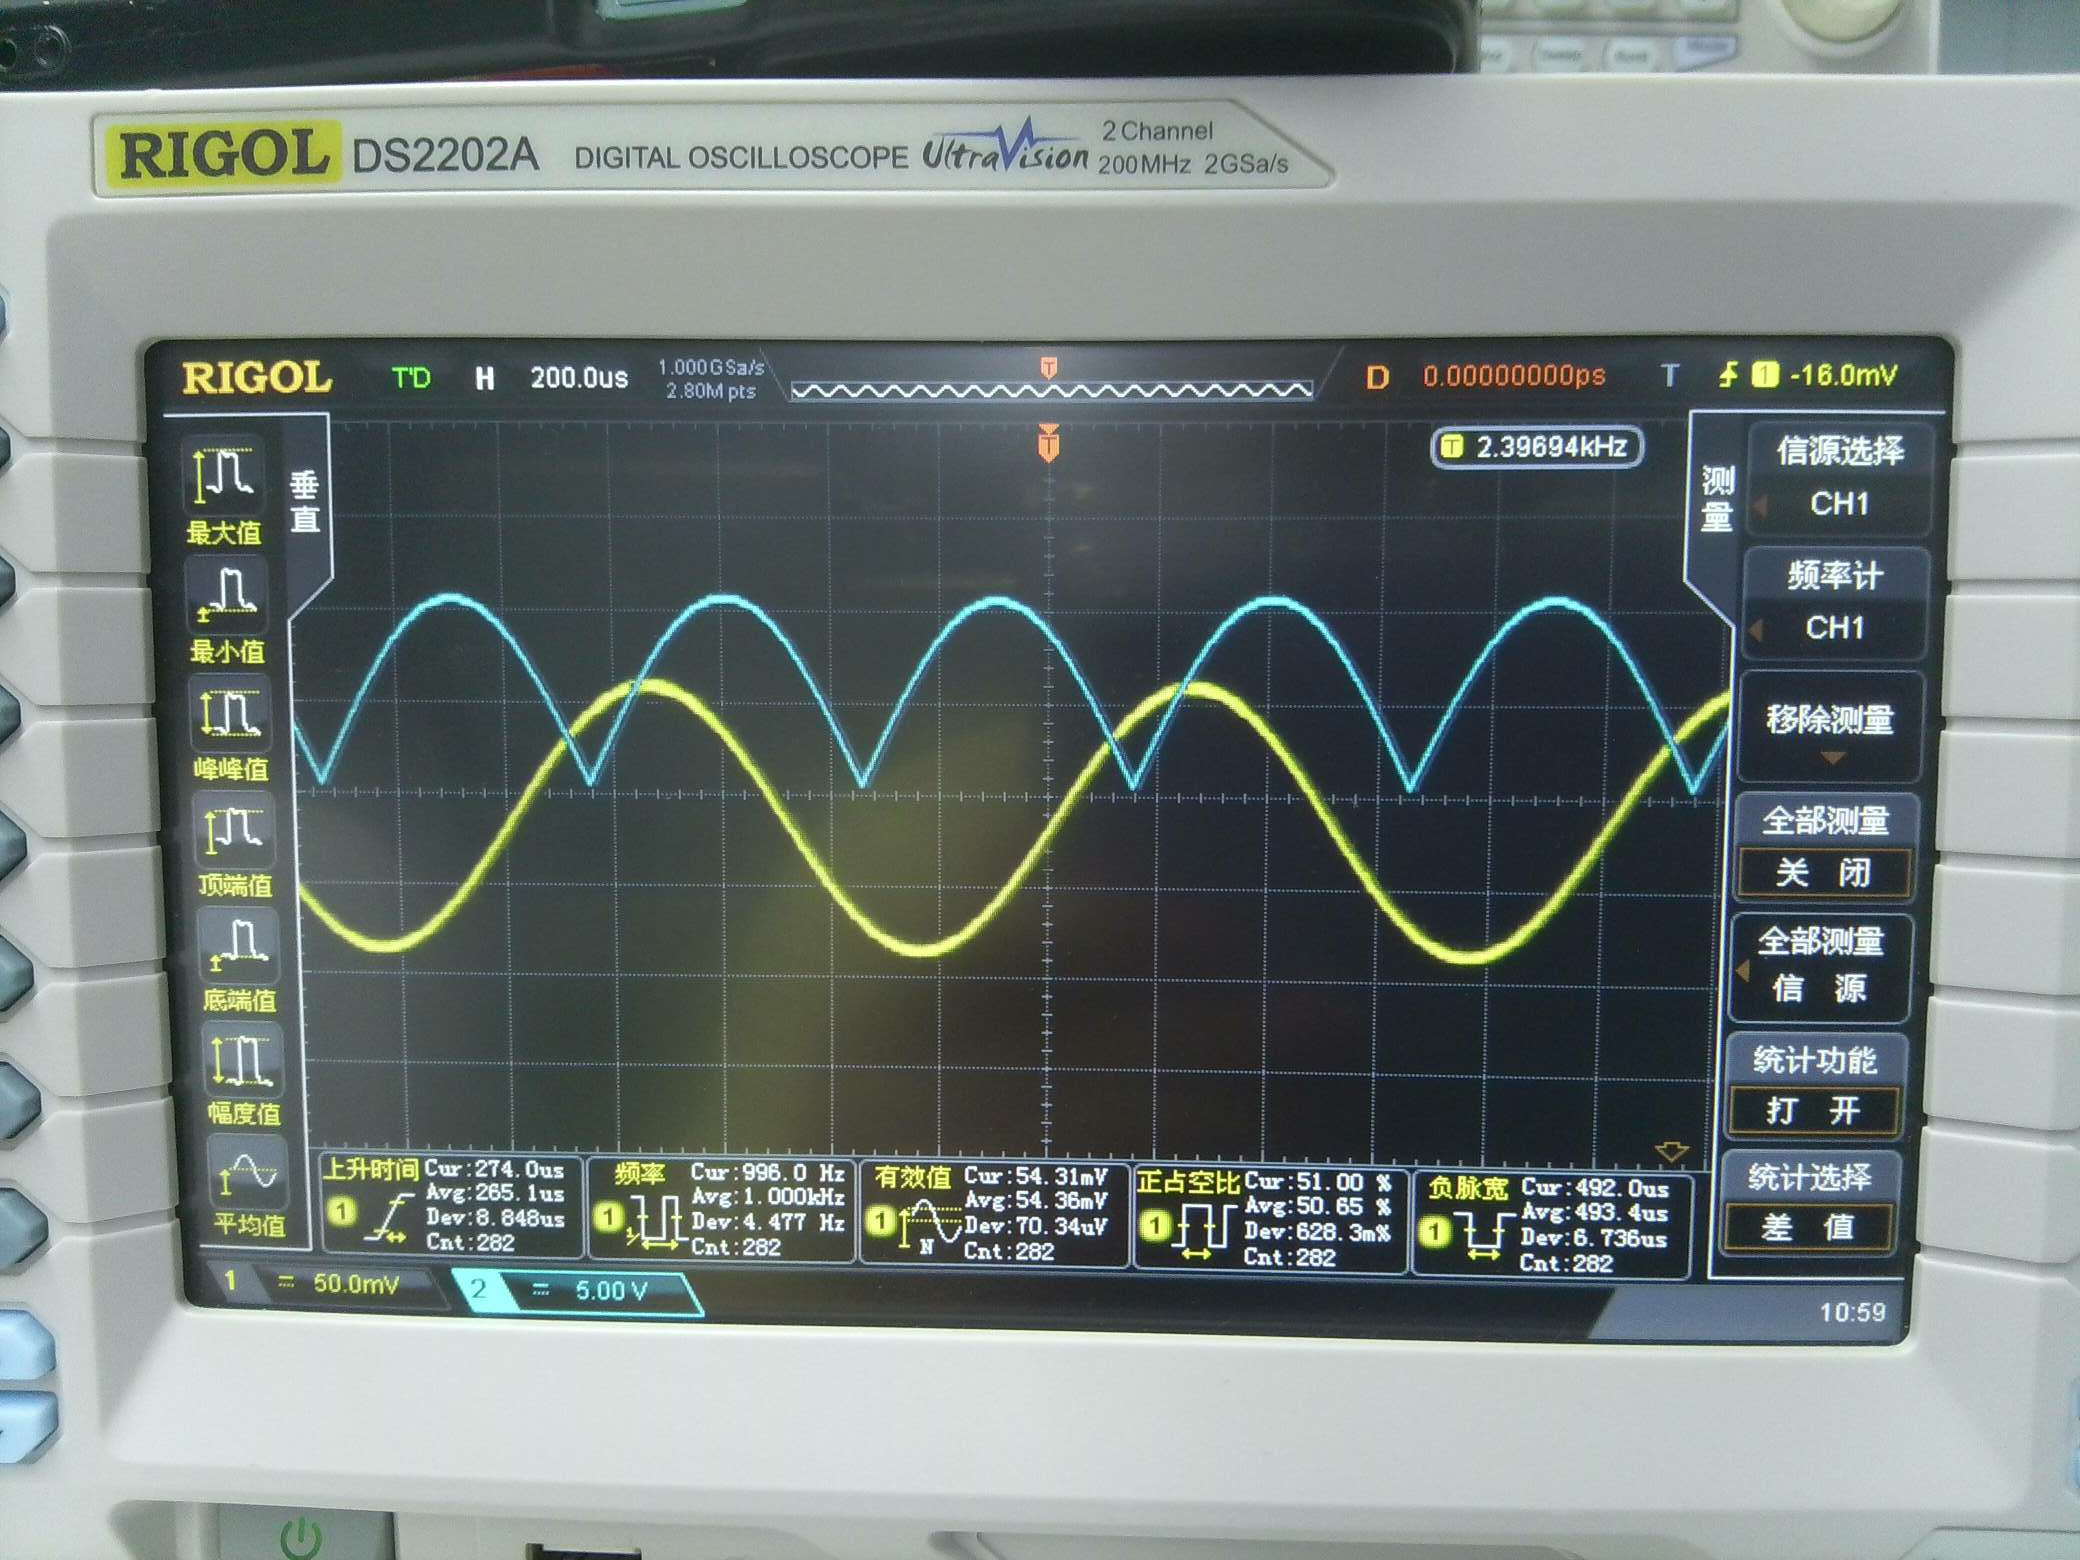
\includegraphics[width=3cm]{示波器图片1.1.png} & \includegraphics[width=3cm]{1.2.png}&\includegraphics[width=3cm]{1.3.png} \\
				\hline
				% 数据行 2
				100us &\includegraphics[width=3cm]{2.1.png} & \includegraphics[width=3cm]{2.2.png} & \includegraphics[width=3cm]{2.3.png}\\
				
				\hline
				% 数据行 3
				1ms &\includegraphics[width=3cm]{3.1.png} & \includegraphics[width=3cm]{3.2.png} & 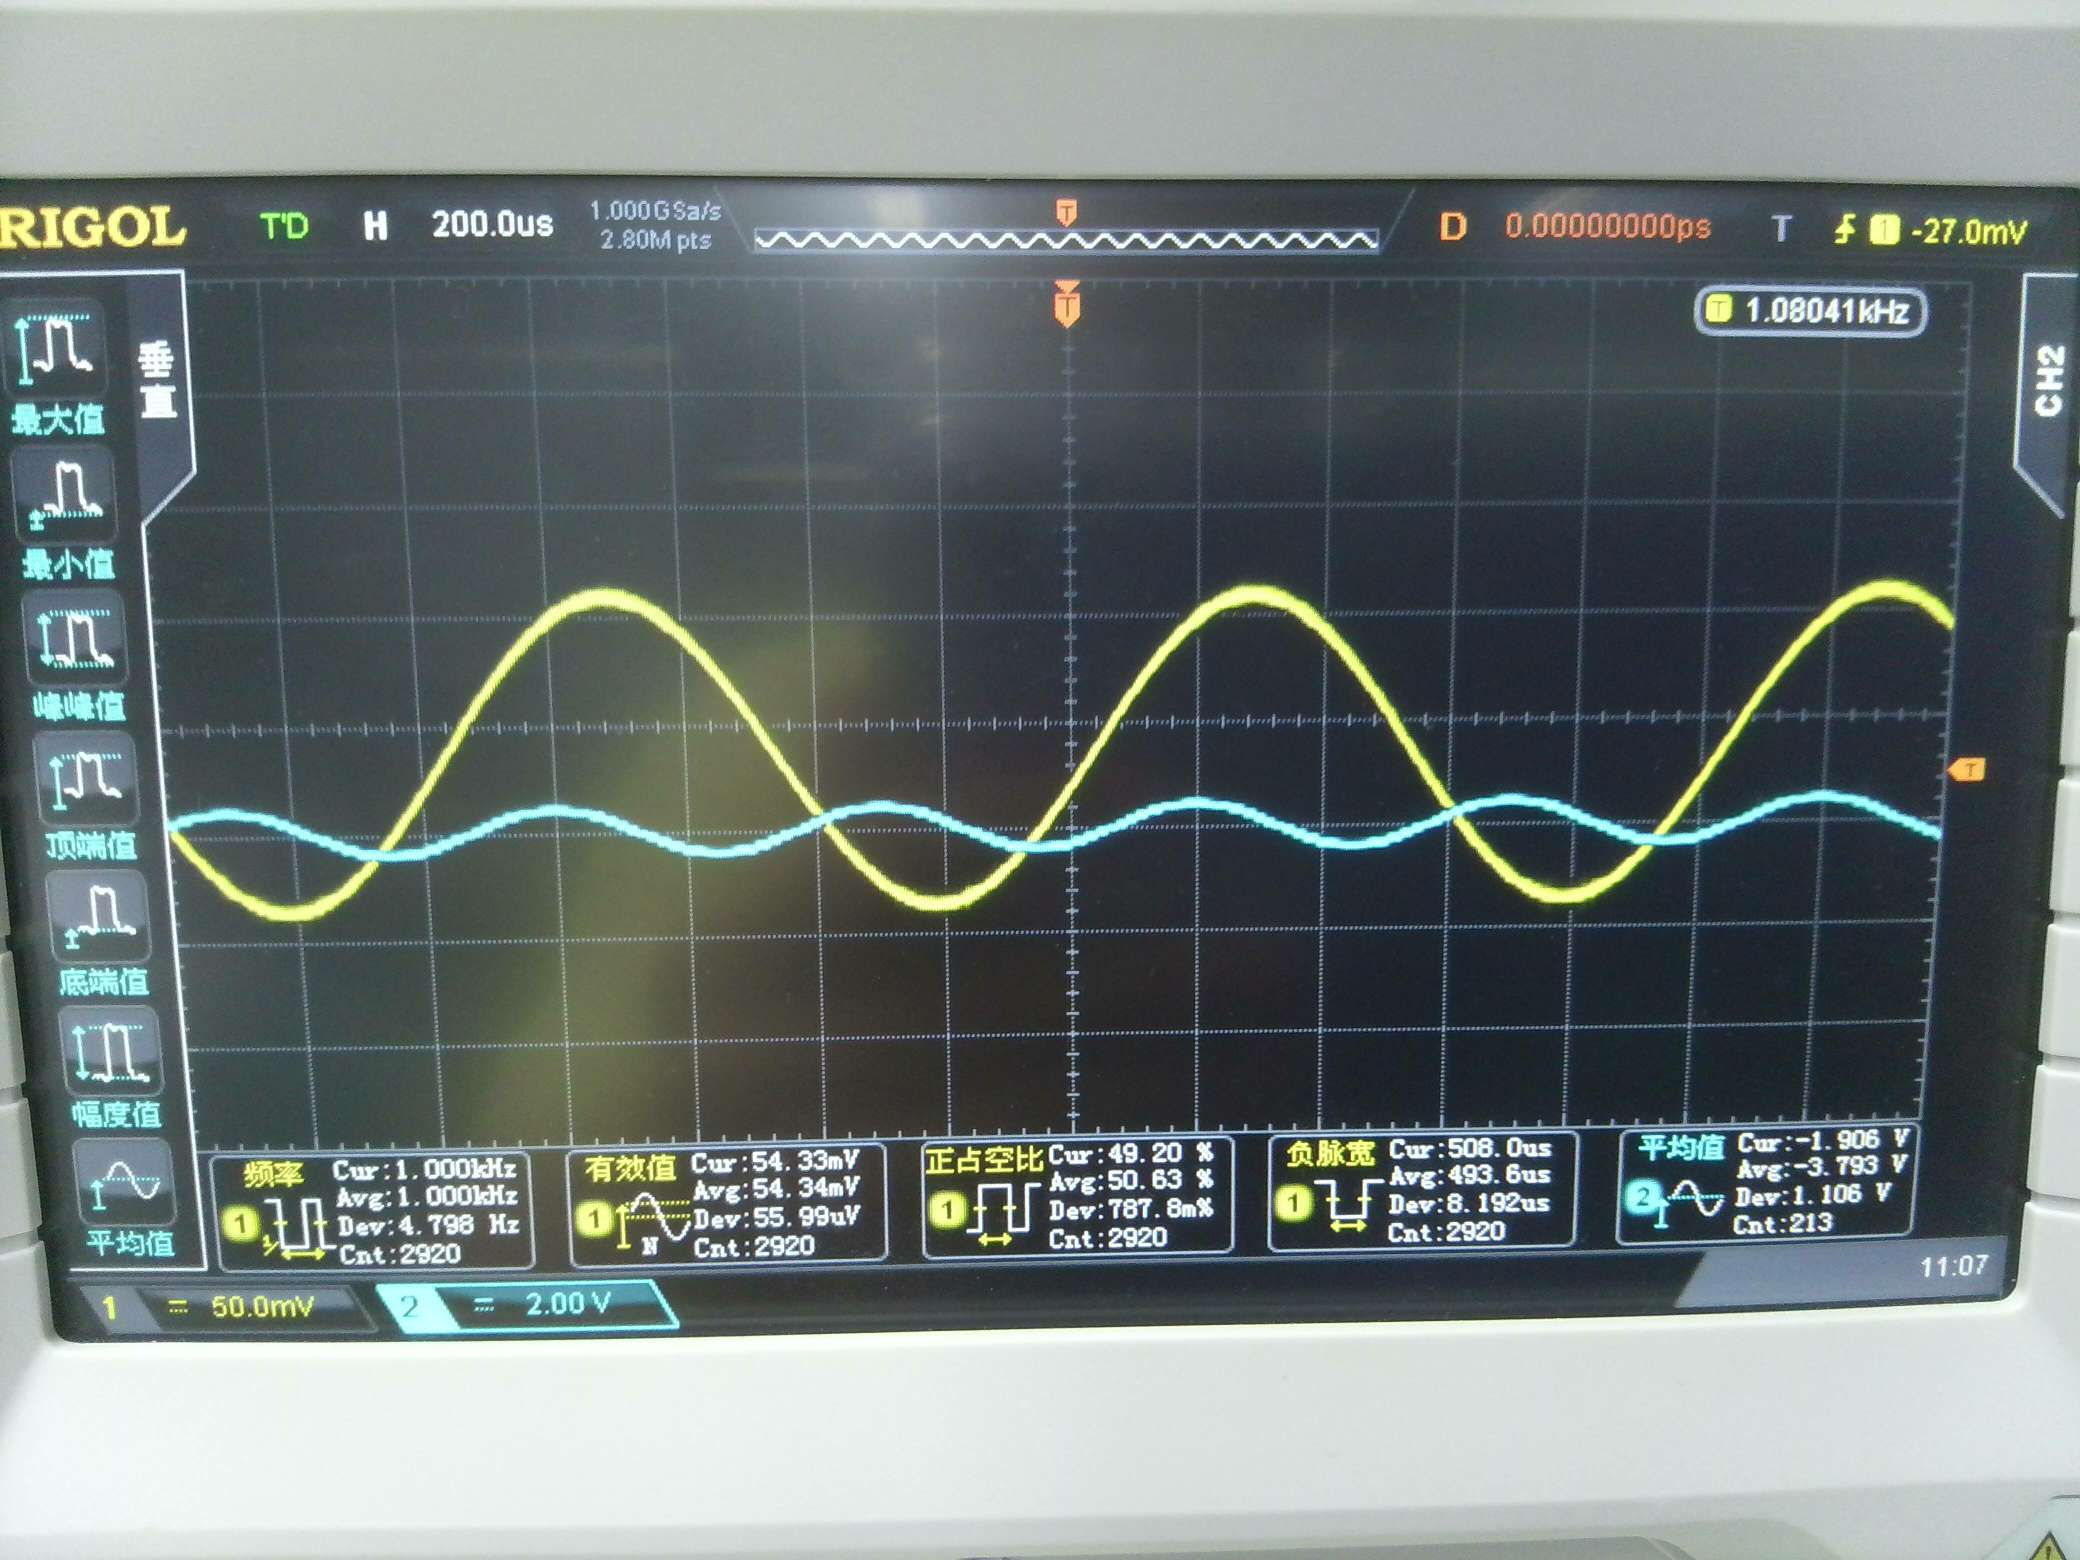
\includegraphics[width=3cm]{3.3.png} \\
				
				\hline
				% 数据行 4
				10ms & \includegraphics[width=3cm]{4.1.png} & \includegraphics[width=3cm]{4.2.png} & \includegraphics[width=3cm]{4.3.png} \\
				
				\hline
				% 数据行 5
				100ms & \includegraphics[width=3cm]{5.1.png} & \includegraphics[width=3cm]{5.2.png} & \includegraphics[width=3cm]{5.3.png} \\
				
				\hline
				% 数据行 6
				1s & 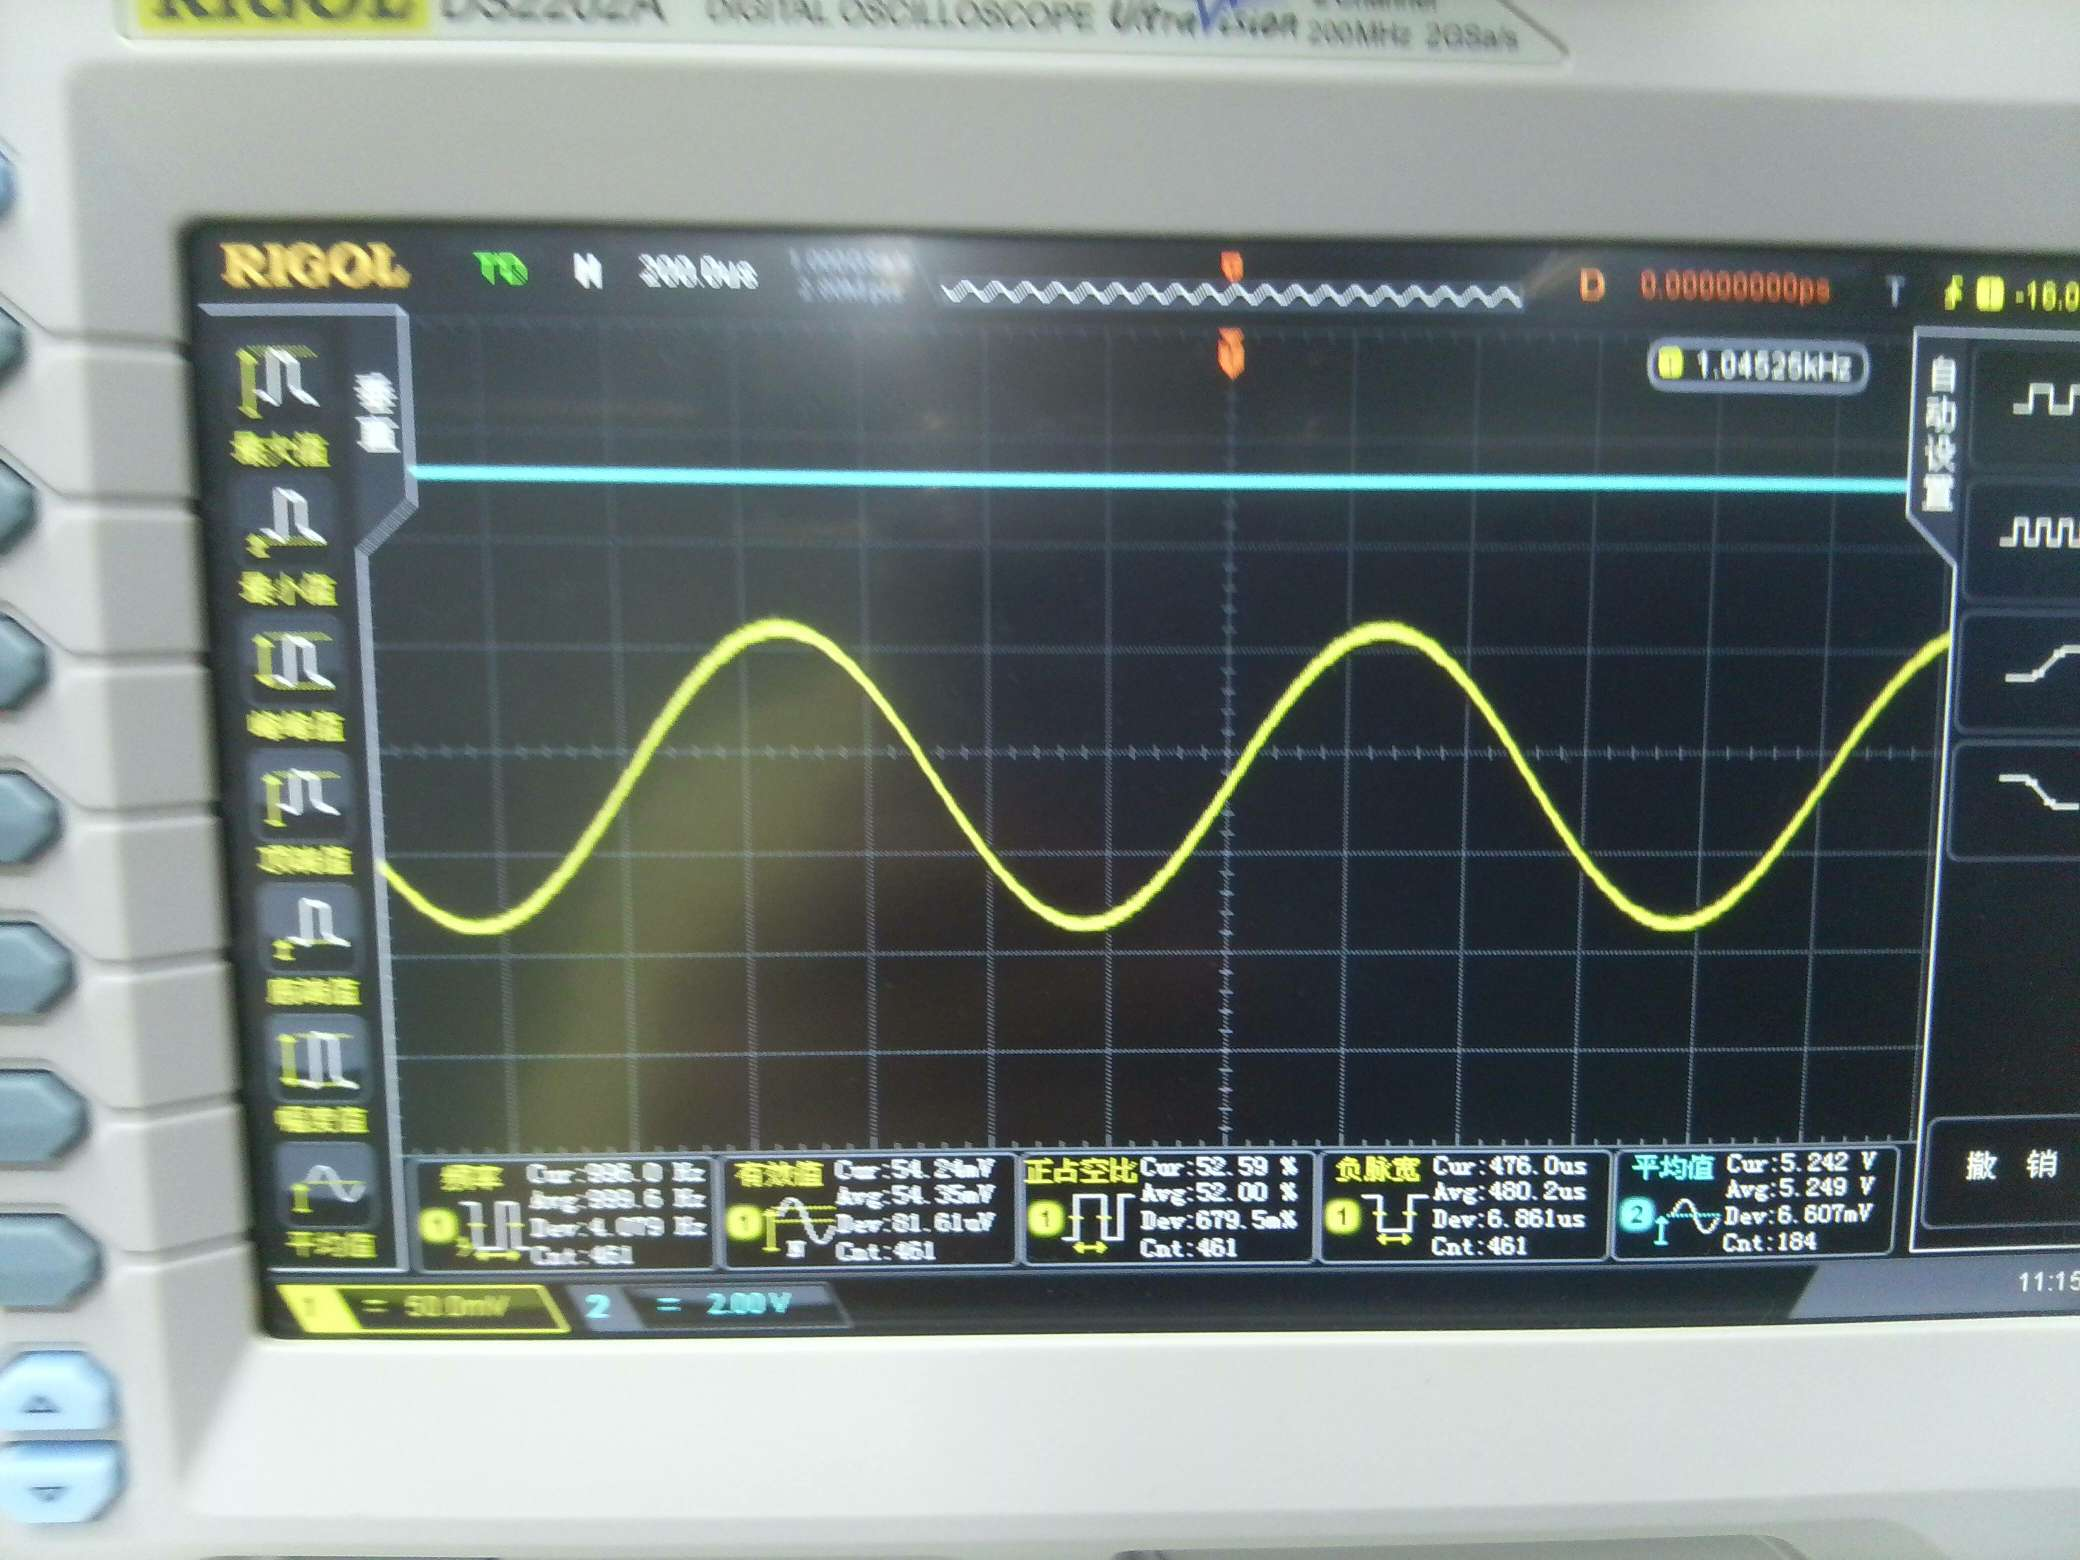
\includegraphics[width=3cm]{6.1.png} & \includegraphics[width=3cm]{6.2.png}  & \includegraphics[width=3cm]{6.3.png} \\
				
				\hline
		\end{tabularx}
		\caption{陡降为6dB/oct时,改变时间常数,低通滤波器配合乘法器解调过程探究记录}
		\label{tab:1}
		\end{table}
		
		\begin{table}[ht]
			\centering
			\begin{tabularx}{\textwidth}{|c|X|X|X|}
				\hline
				% 第一行表头
				陡降(dB/oct) & R波形  & X波形  & Y波形 \\
				\hline
				% 数据行 1
				6 & \includegraphics[width=3cm]{D1.1.png} & \includegraphics[width=3cm]{D1.2.png} &\includegraphics[width=3cm]{D1.3.png}\\
				\hline
				% 数据行 2
				12 & \includegraphics[width=3cm]{D2.1.png}  & \includegraphics[width=3cm]{D2.2.png}  & \includegraphics[width=3cm]{D2.3.png} \\
				\hline
				% 数据行 3
				18 & \includegraphics[width=3cm]{D3.1.png}  & \includegraphics[width=3cm]{D3.2.png}   & \includegraphics[width=3cm]{D3.3.png}   \\
				\hline
				% 数据行 4
				24 & \includegraphics[width=3cm]{D4.1.png}   & \includegraphics[width=3cm]{D4.2.png}   & \includegraphics[width=3cm]{D4.3.png}  \\
				\hline
			\end{tabularx}
			\caption{时间常数TC=100us时,改变陡降,低通滤波器配合乘法器解调过程探究记录}
			\label{tab:2}
			\end{table}

	\subsubsection{滤波器带宽对输出信号响应的影响}
			\begin{enumerate}
				\item 设置待测信号幅值从$V_1$瞬间变化到$V_2$,本实验信号变化为0.1-0.6m$V_{rms}$。
				\item 选择量程灵敏度为大信号,使得信号$V_1$与$V_2$在锁相放大器的量程内。
				\item 设置不同大小的时间常数,观察并记录锁相放大器的输出信号R,与输入信号变化随时间变化的响应。
				\item 试验观测图像整理如表\ref{tab:3}。
			\end{enumerate}

			\begin{table}[ht]
				\centering
				\begin{tabularx}{\textwidth}{|X|X|}
					\hline
					% 第一行
					时间常数TC & R对信号变化(0.1-0.6m$V_{rms}$)的响应变化 \\
					\hline
					% 第二行
					1S & 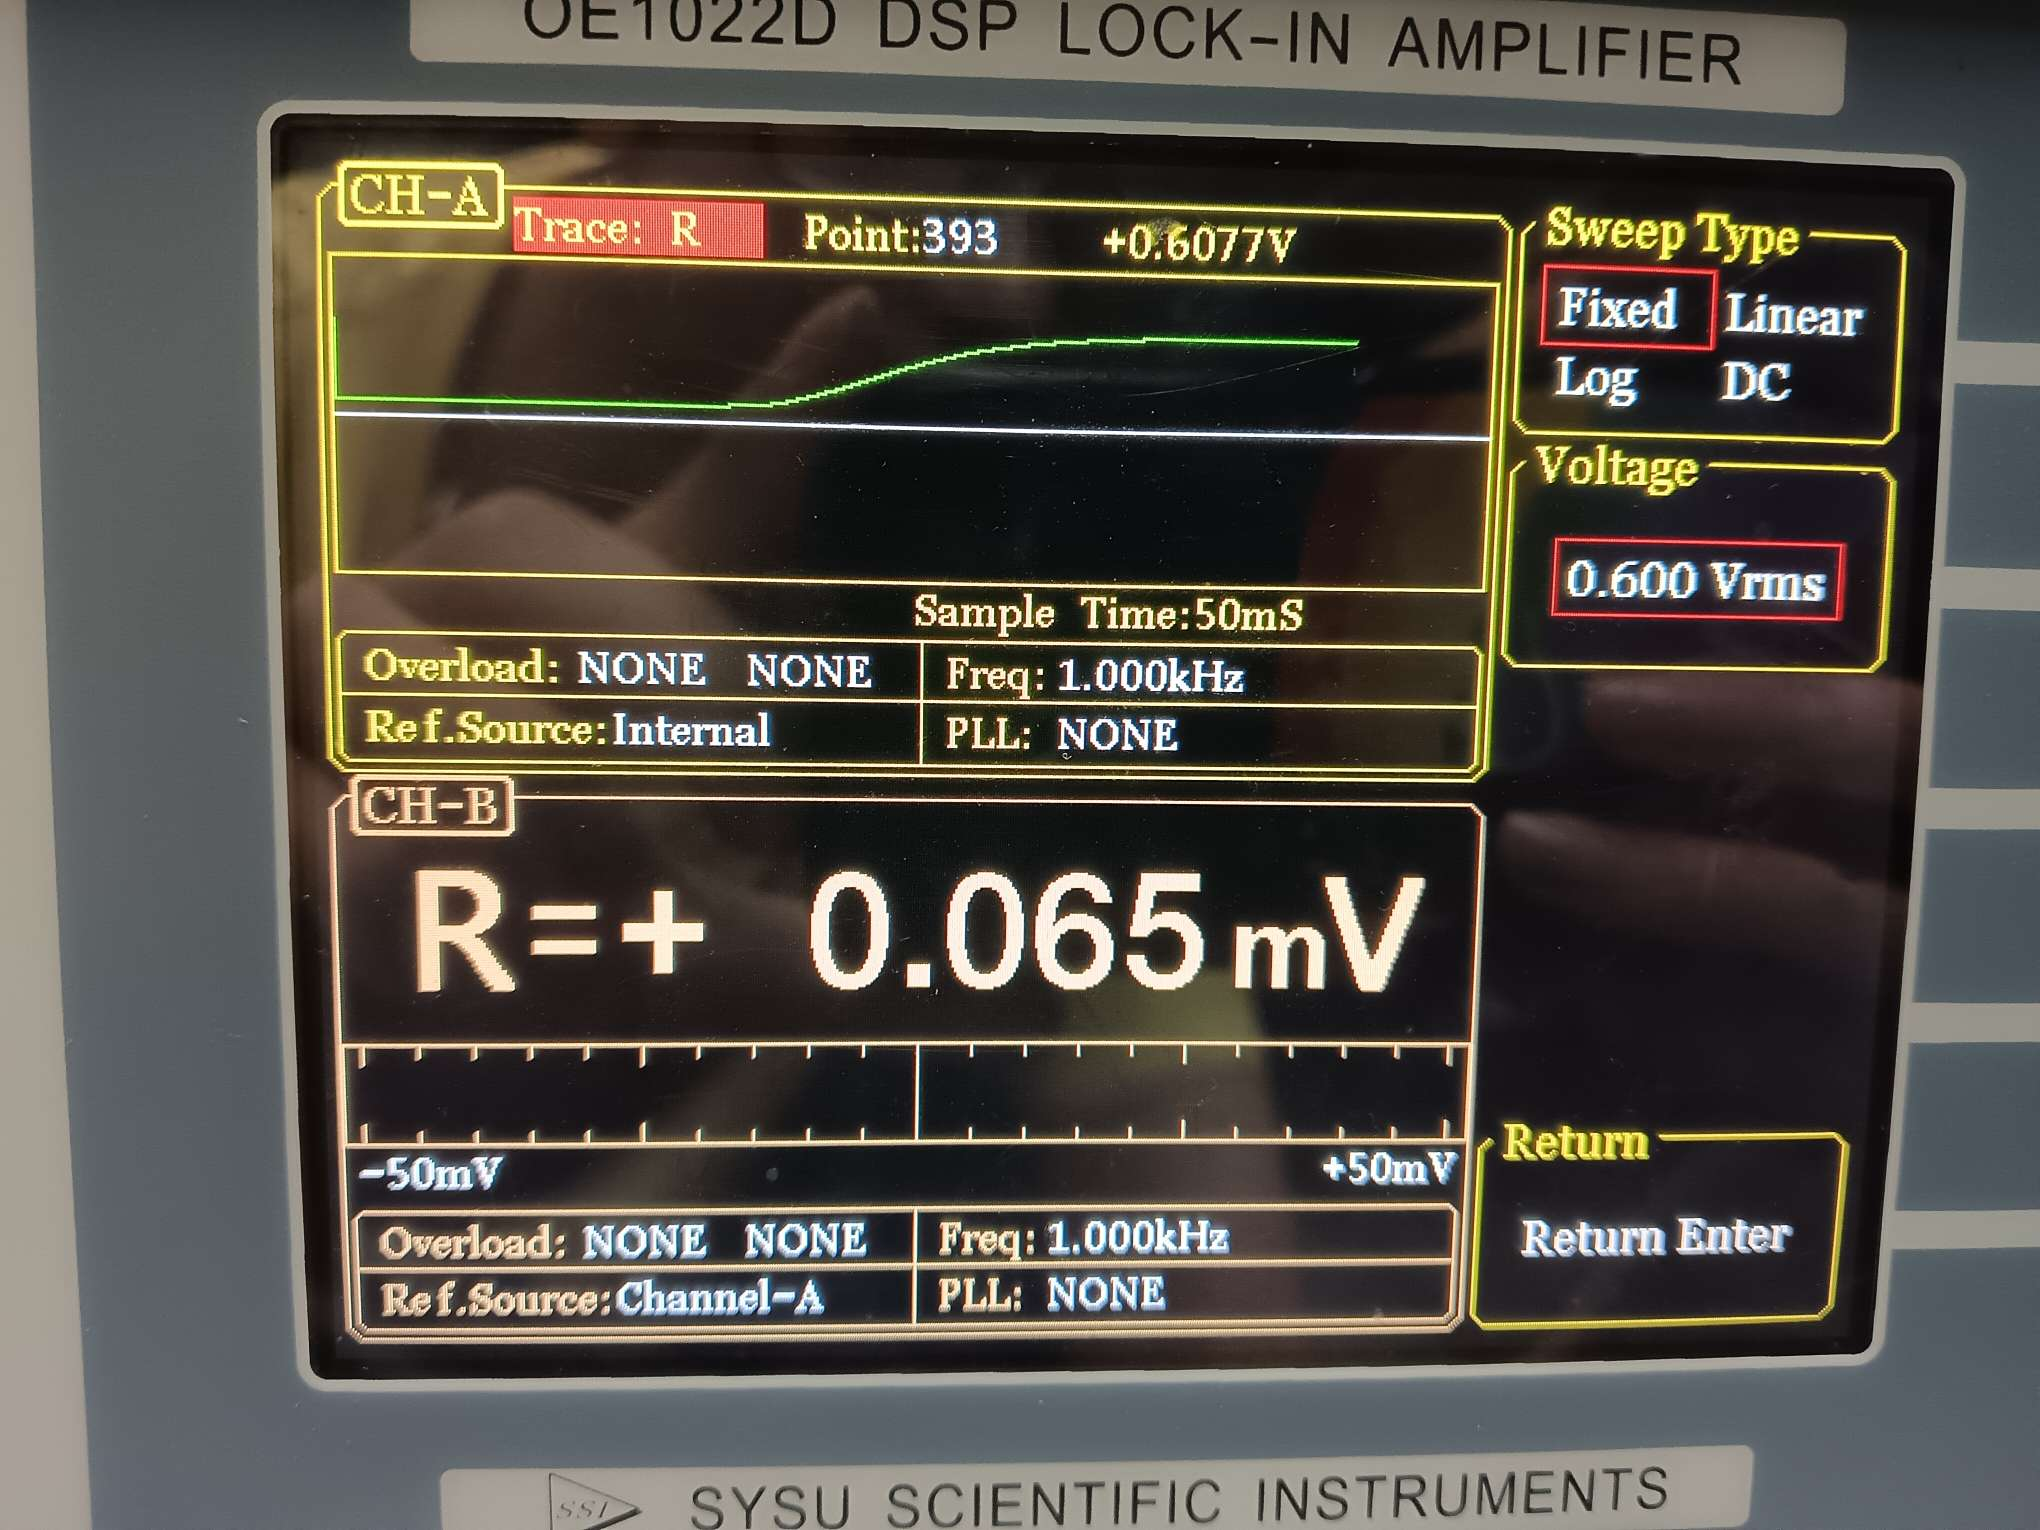
\includegraphics[width=3cm]{R1.1.png}    \\
					\hline
					% 第三行
					10mS& 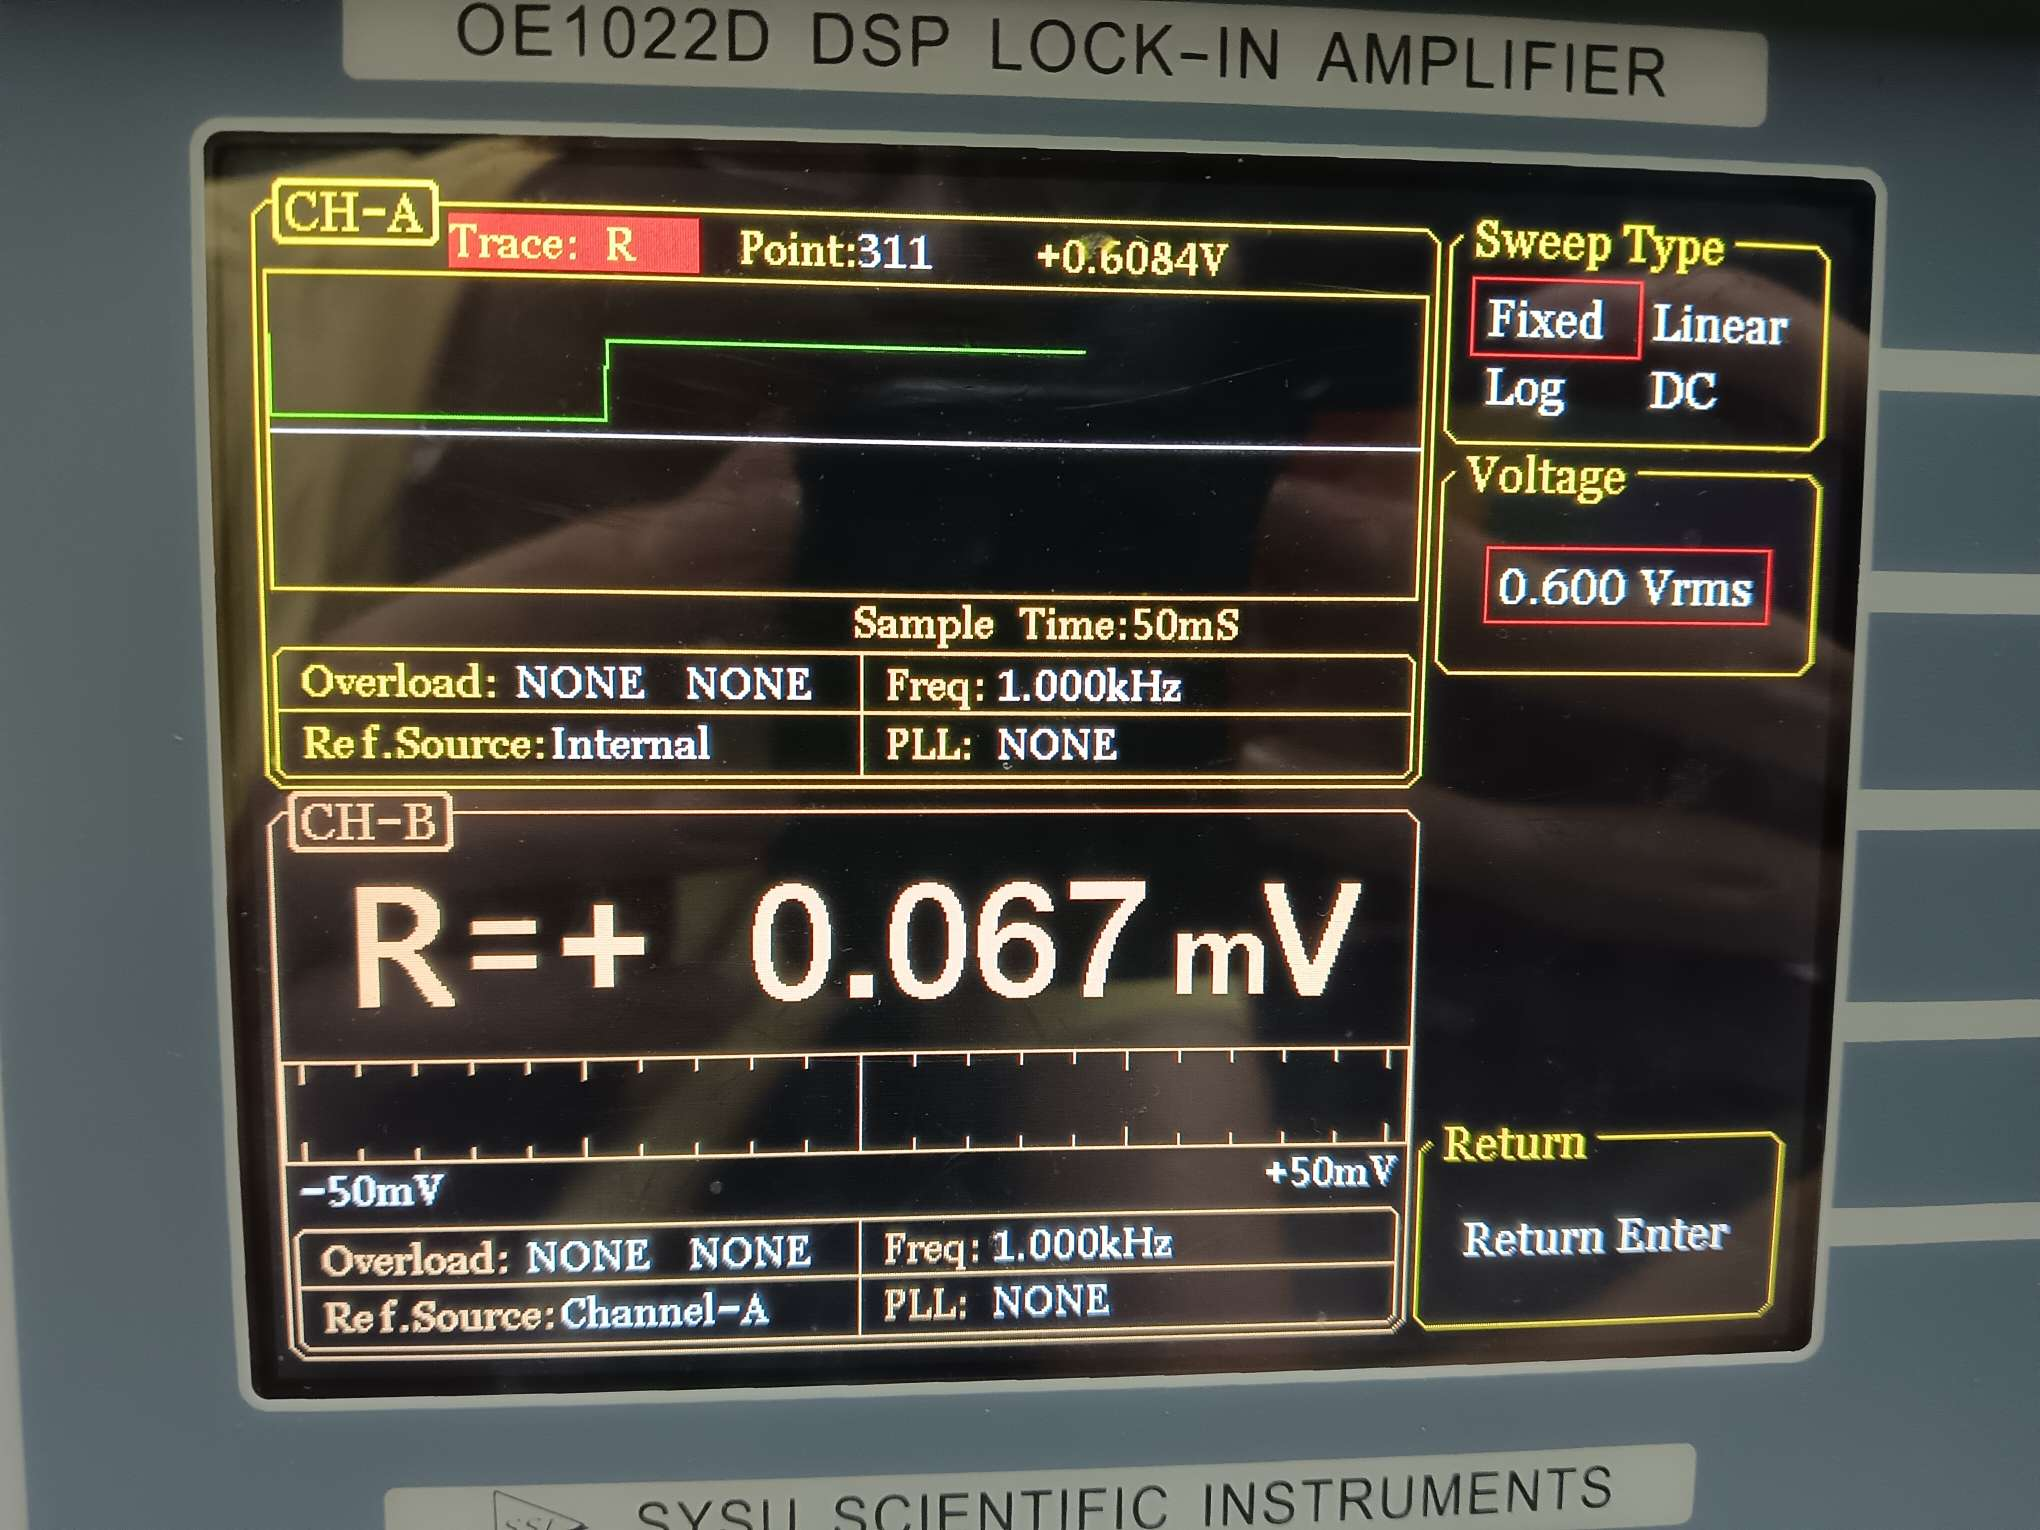
\includegraphics[width=3cm]{R2.1.png}     \\
					\hline
					% 第四行
					300mS &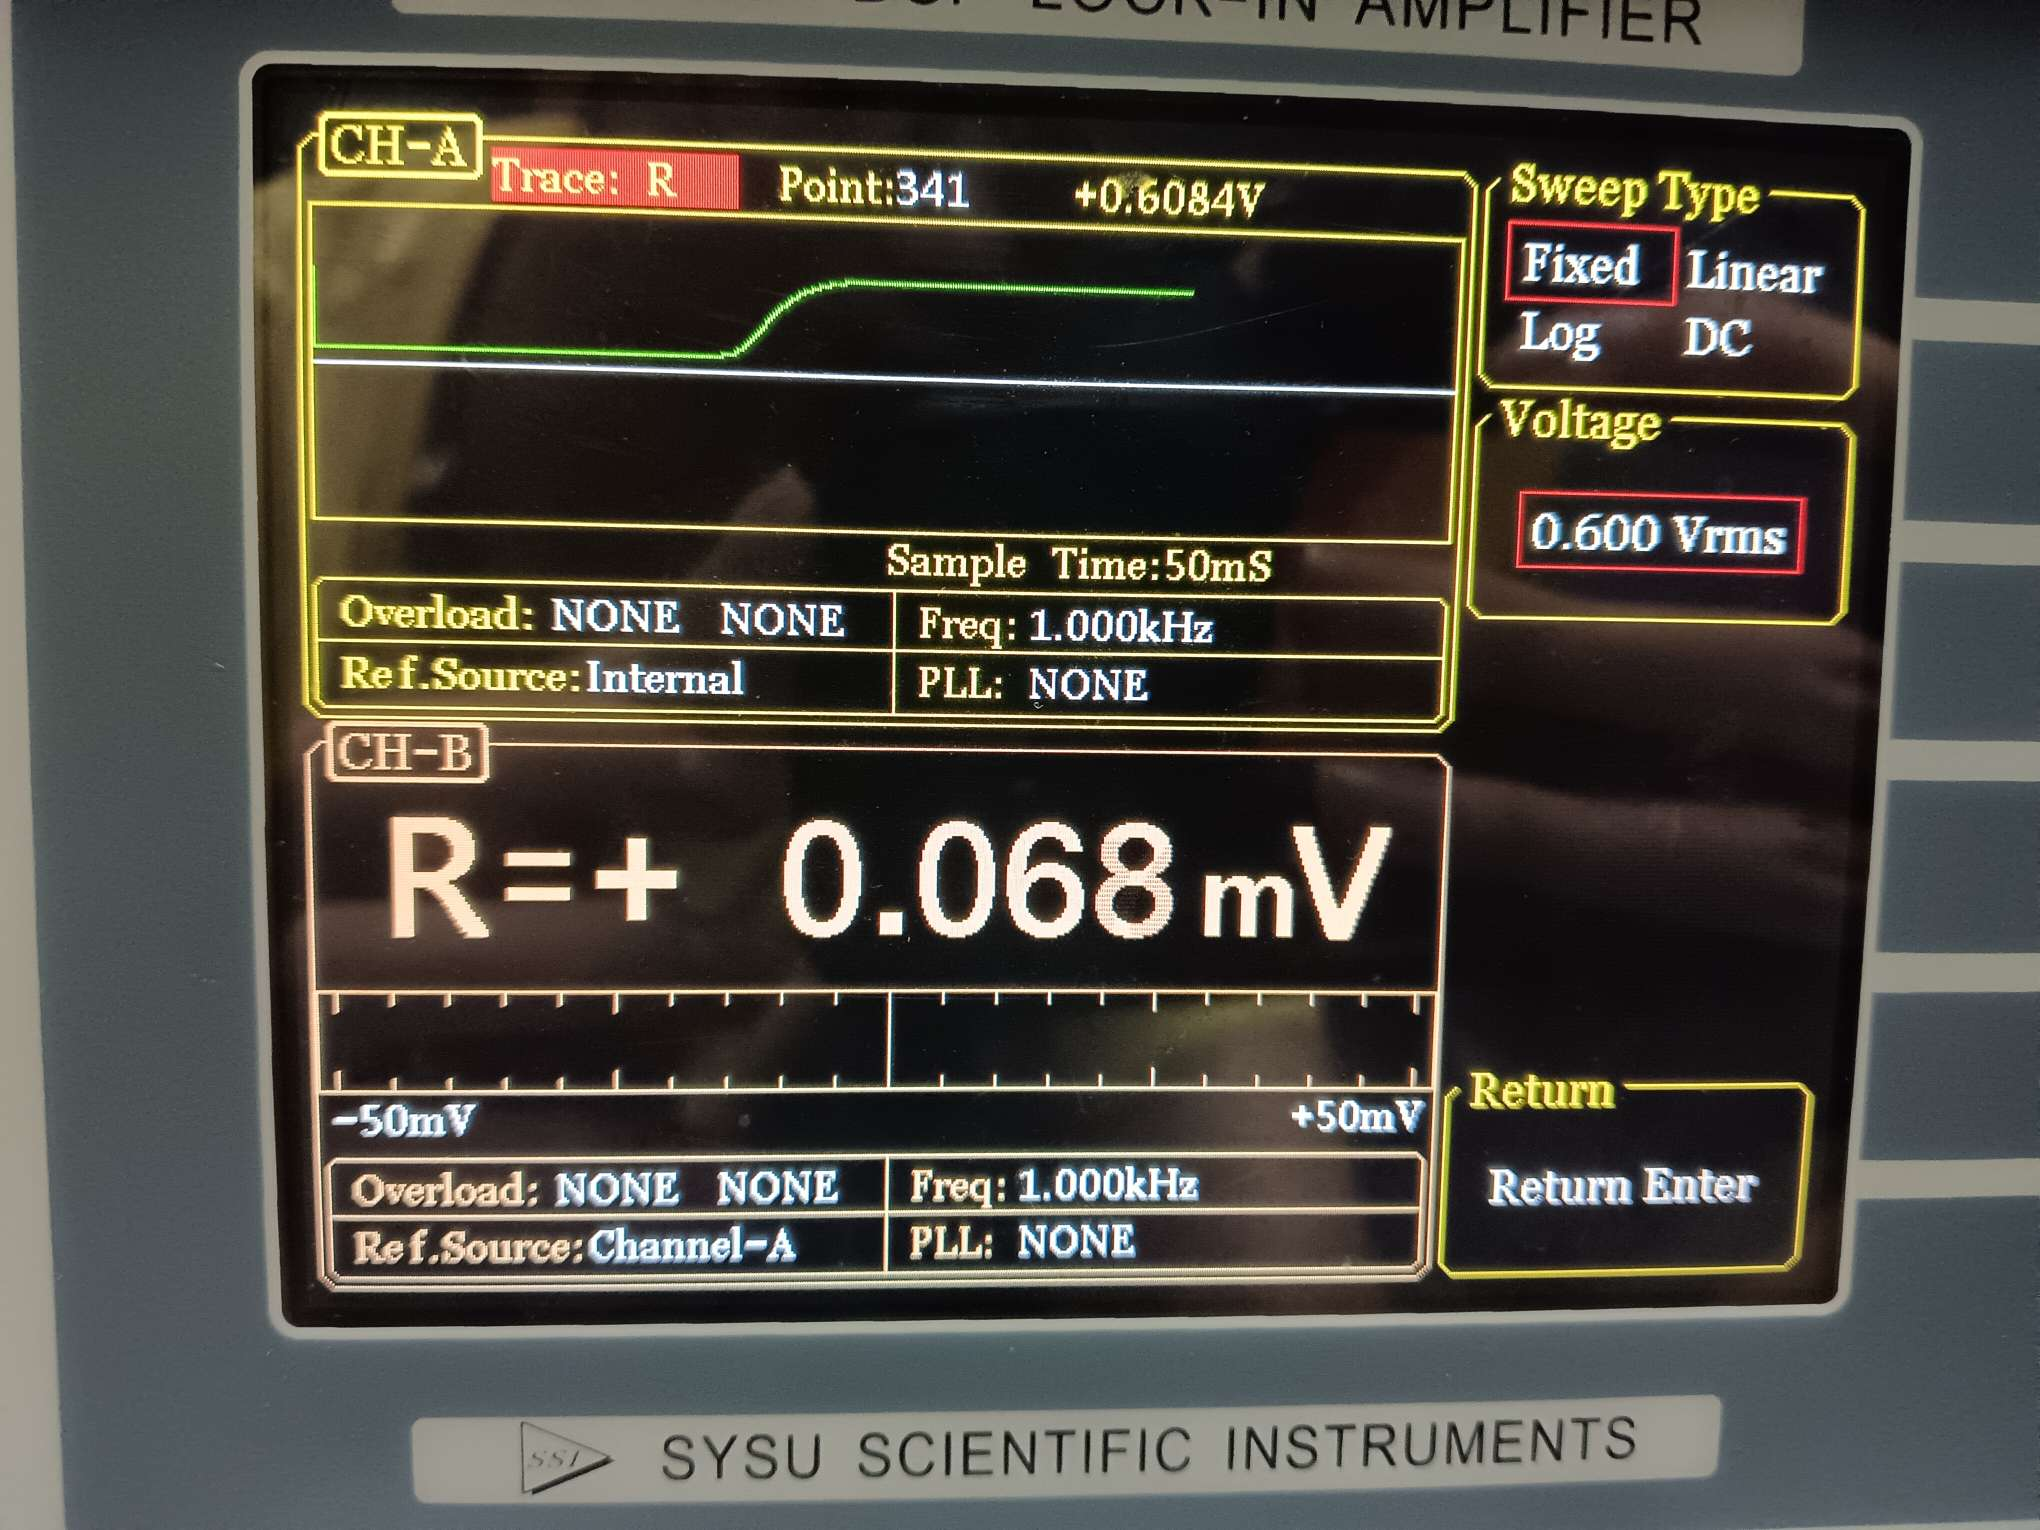
\includegraphics[width=3cm]{R3.1.png}    \\
					\hline
					% 第五行
					100mS & \includegraphics[width=3cm]{R4.1.png}     \\
					\hline
				\end{tabularx}
				\caption{陡降为24dB/oct时,不同大小的时间常数,锁相放大器输出波形}
				\label{tab:3}
				\end{table}

	\subsubsection{强噪声背景下的弱信号检测}
		\begin{enumerate}
			\item 将教学实验箱噪声发生器通电,使用示波器观察并记录教学实验箱的输出信号,同时记录时域与频域图谱,如图\ref{fig:测量实验箱输出的噪声的频率与时域图谱}所示。从图中可以得到:实验箱输出的是白噪声,因为噪声的时域与频域图谱都表现为随机特征。
			\item 设置信号发生器的频率为非市电倍频(986Hz),幅值适当的正弦波信号与噪声信号叠加。
			\item 调节锁相放大器的量程灵敏度与LPF带宽,获得至少两位的稳定数字的读数(尽量记录为三位有效数字),并记录R值与对应的锁相放大器参数。
			\item 在示波器中通过“Math”选择带通滤波器,设置信号频段为0.5kHz——1.5kHz,记录滤波后信号的有效值,并截录滤波前后的波形图与所测信号值的波形图。
			\item 改变OE1022产生正弦波的有效值,在不同信噪比下重复测量三种信噪比的情况,其中必须包含信噪比为-60dB的情况。
			\item 实验数据记录如图\ref{tab:强噪声背景下的弱信号检测},观察滤波效果,分析实验结果。
		\end{enumerate}

		\begin{figure}[htbp]
			\centering
			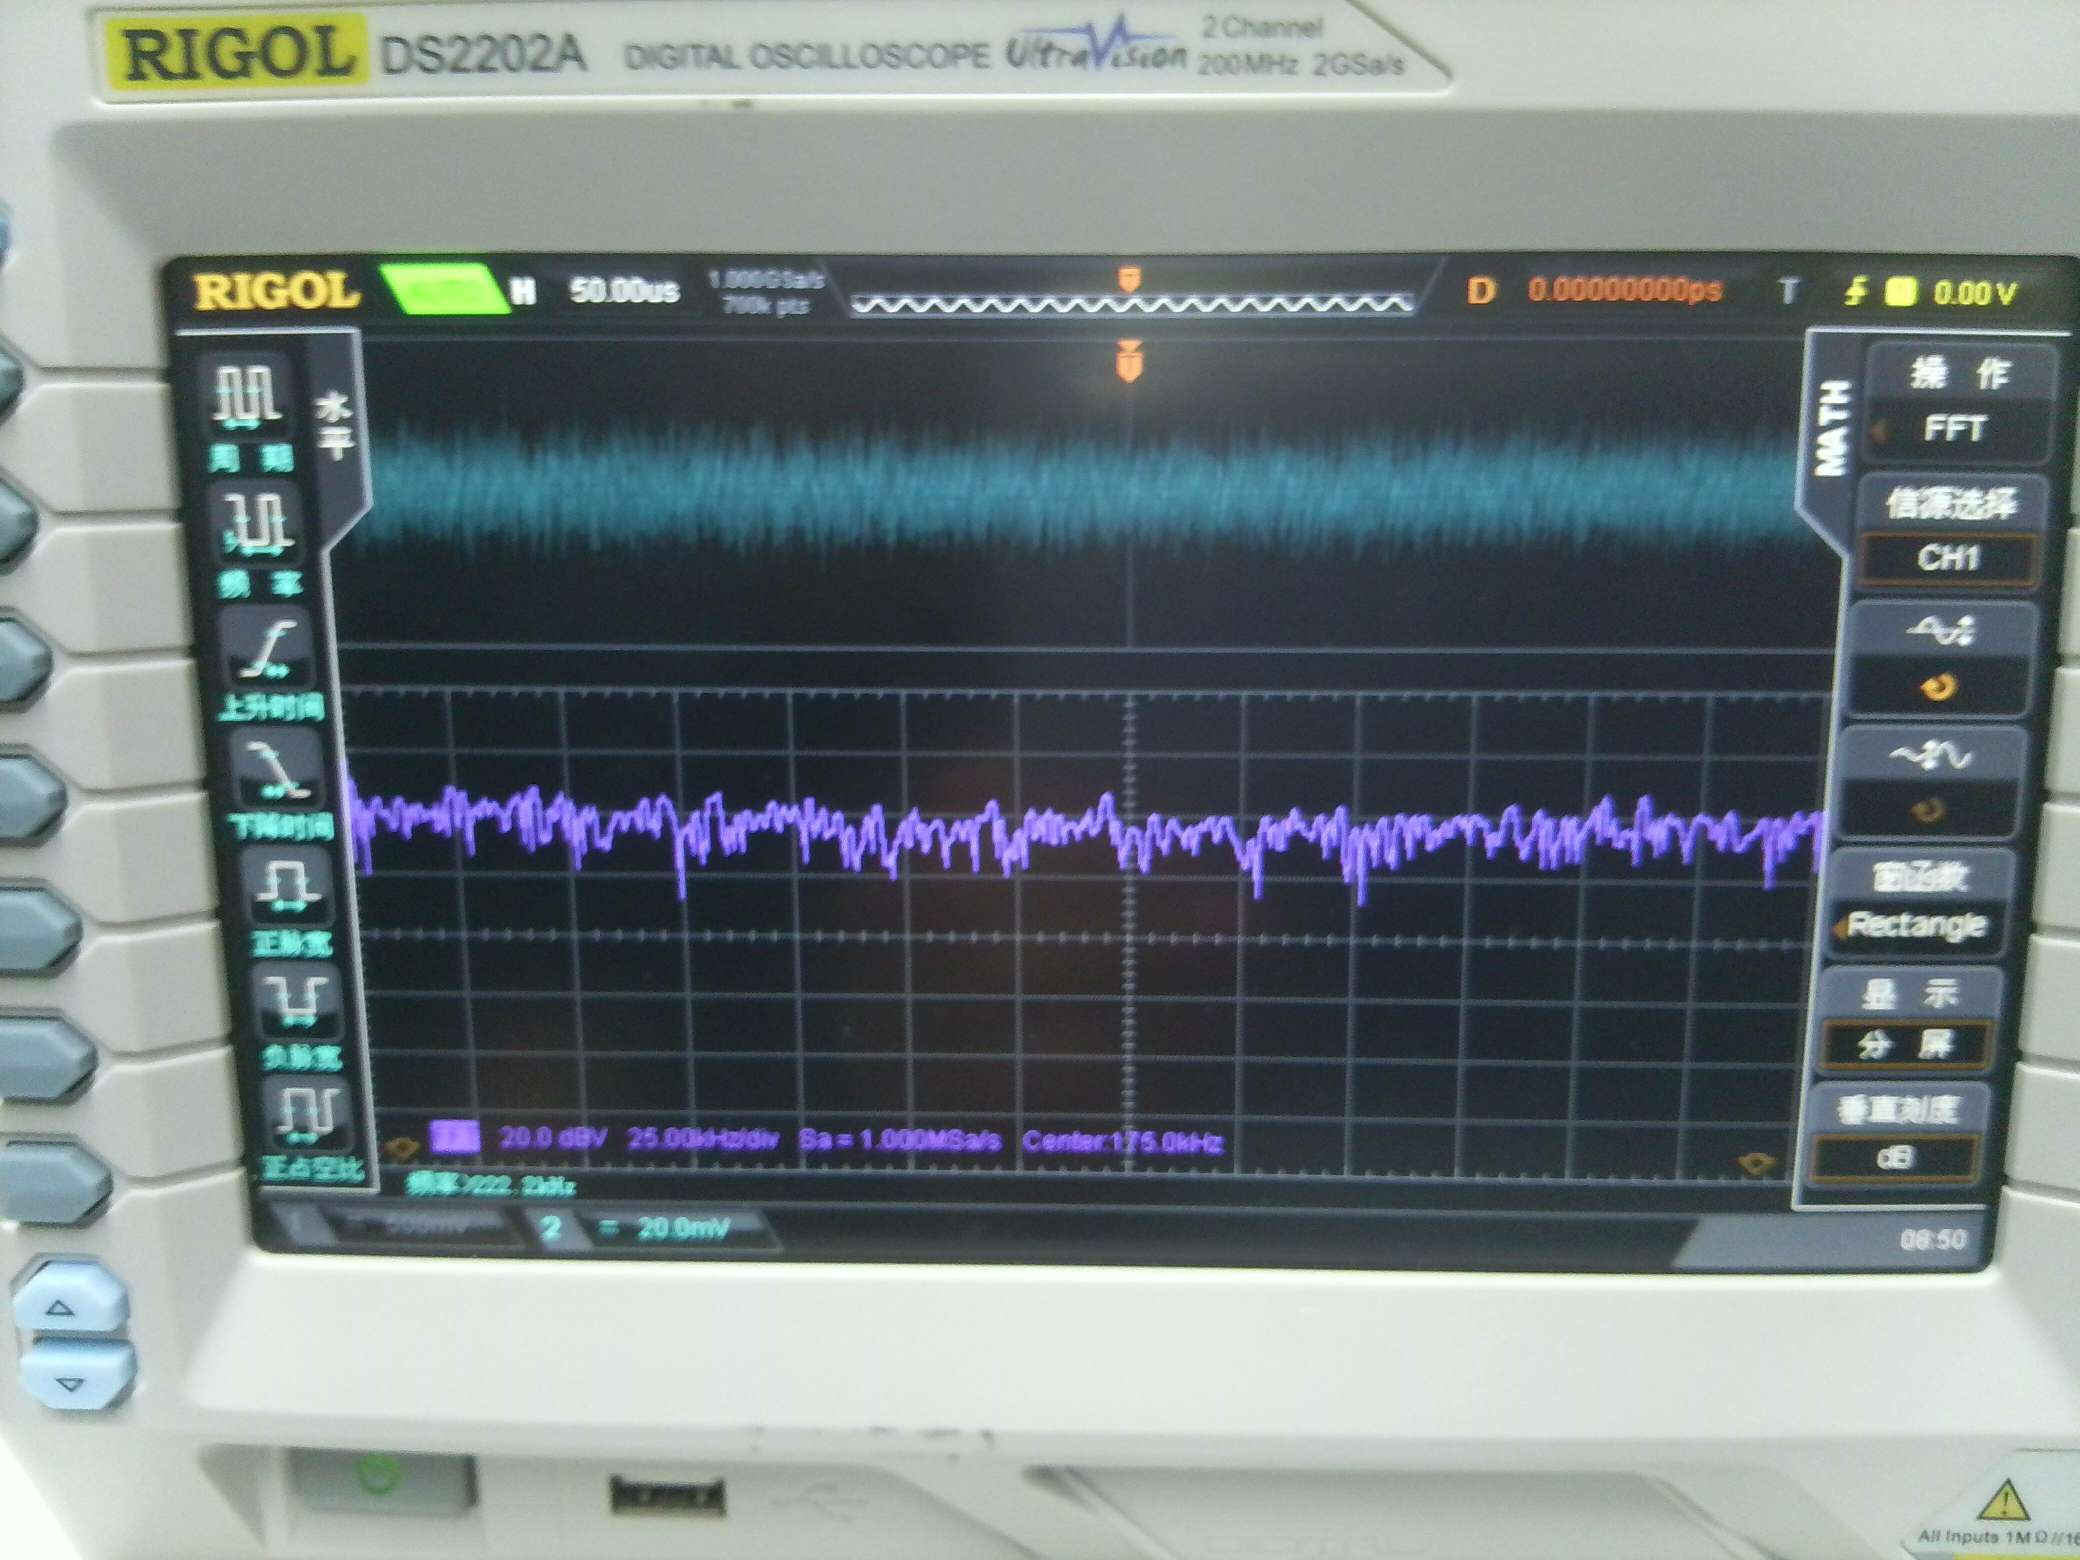
\includegraphics[width=0.75\textwidth]{测量实验箱输出的噪声.png}
			\caption{测量实验箱输出的噪声的频率与时域图谱}
			\label{fig:测量实验箱输出的噪声的频率与时域图谱}
		\end{figure}

		\begin{table}[ht]
			\centering
				\begin{tabularx}{\textwidth}{|X|X|X|X|X|}
					\hline
					% 第一行
					仪器 & 输入信号信噪比(dB) & 0 & -60 & -80 \\
					\hline
					% 第二行
					示波器 & 正弦波$V_in$幅值(m$V_rms$) & 38.2 & 0.0393 &0.00386\\
					\hline
					% 第三行
					& 噪声信号大小(m$V_rms$)& 38.2 & 37.38&36.41 \\
					\hline
					% 第四行
					& $SNR_i$(dB)&0  & -60&-79.49 \\
					\hline
					% 第五行
					& 待测信号$V_in$波形图&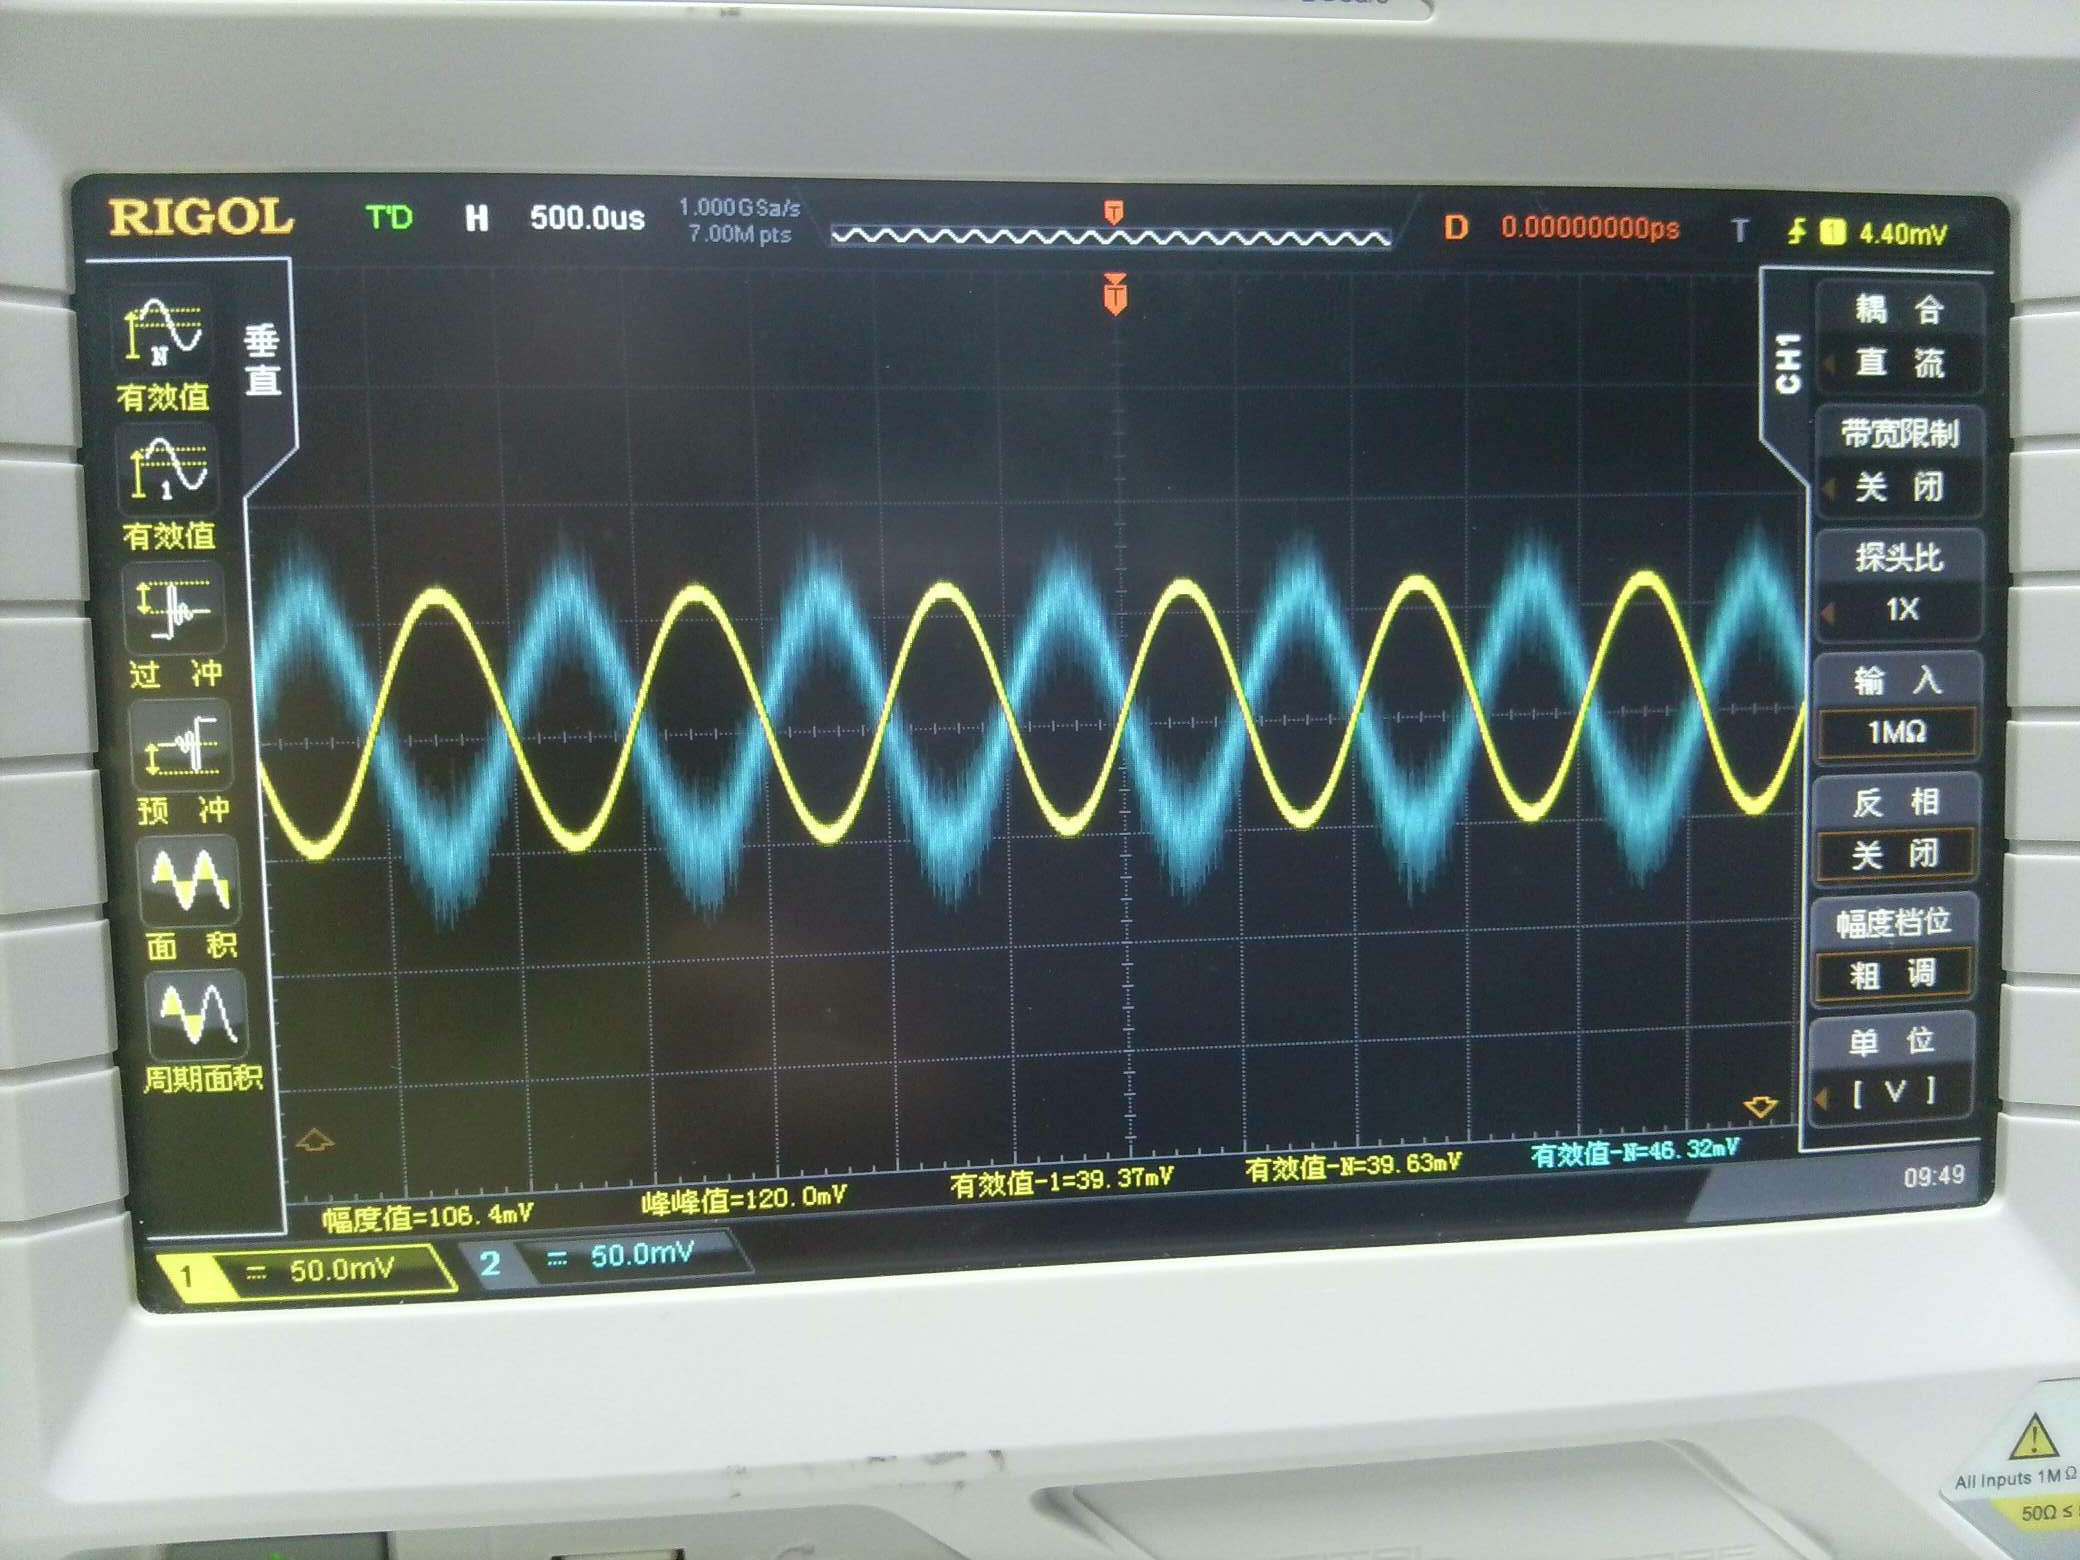
\includegraphics[width=3cm]{待测信号V_in波形图1.png}  & 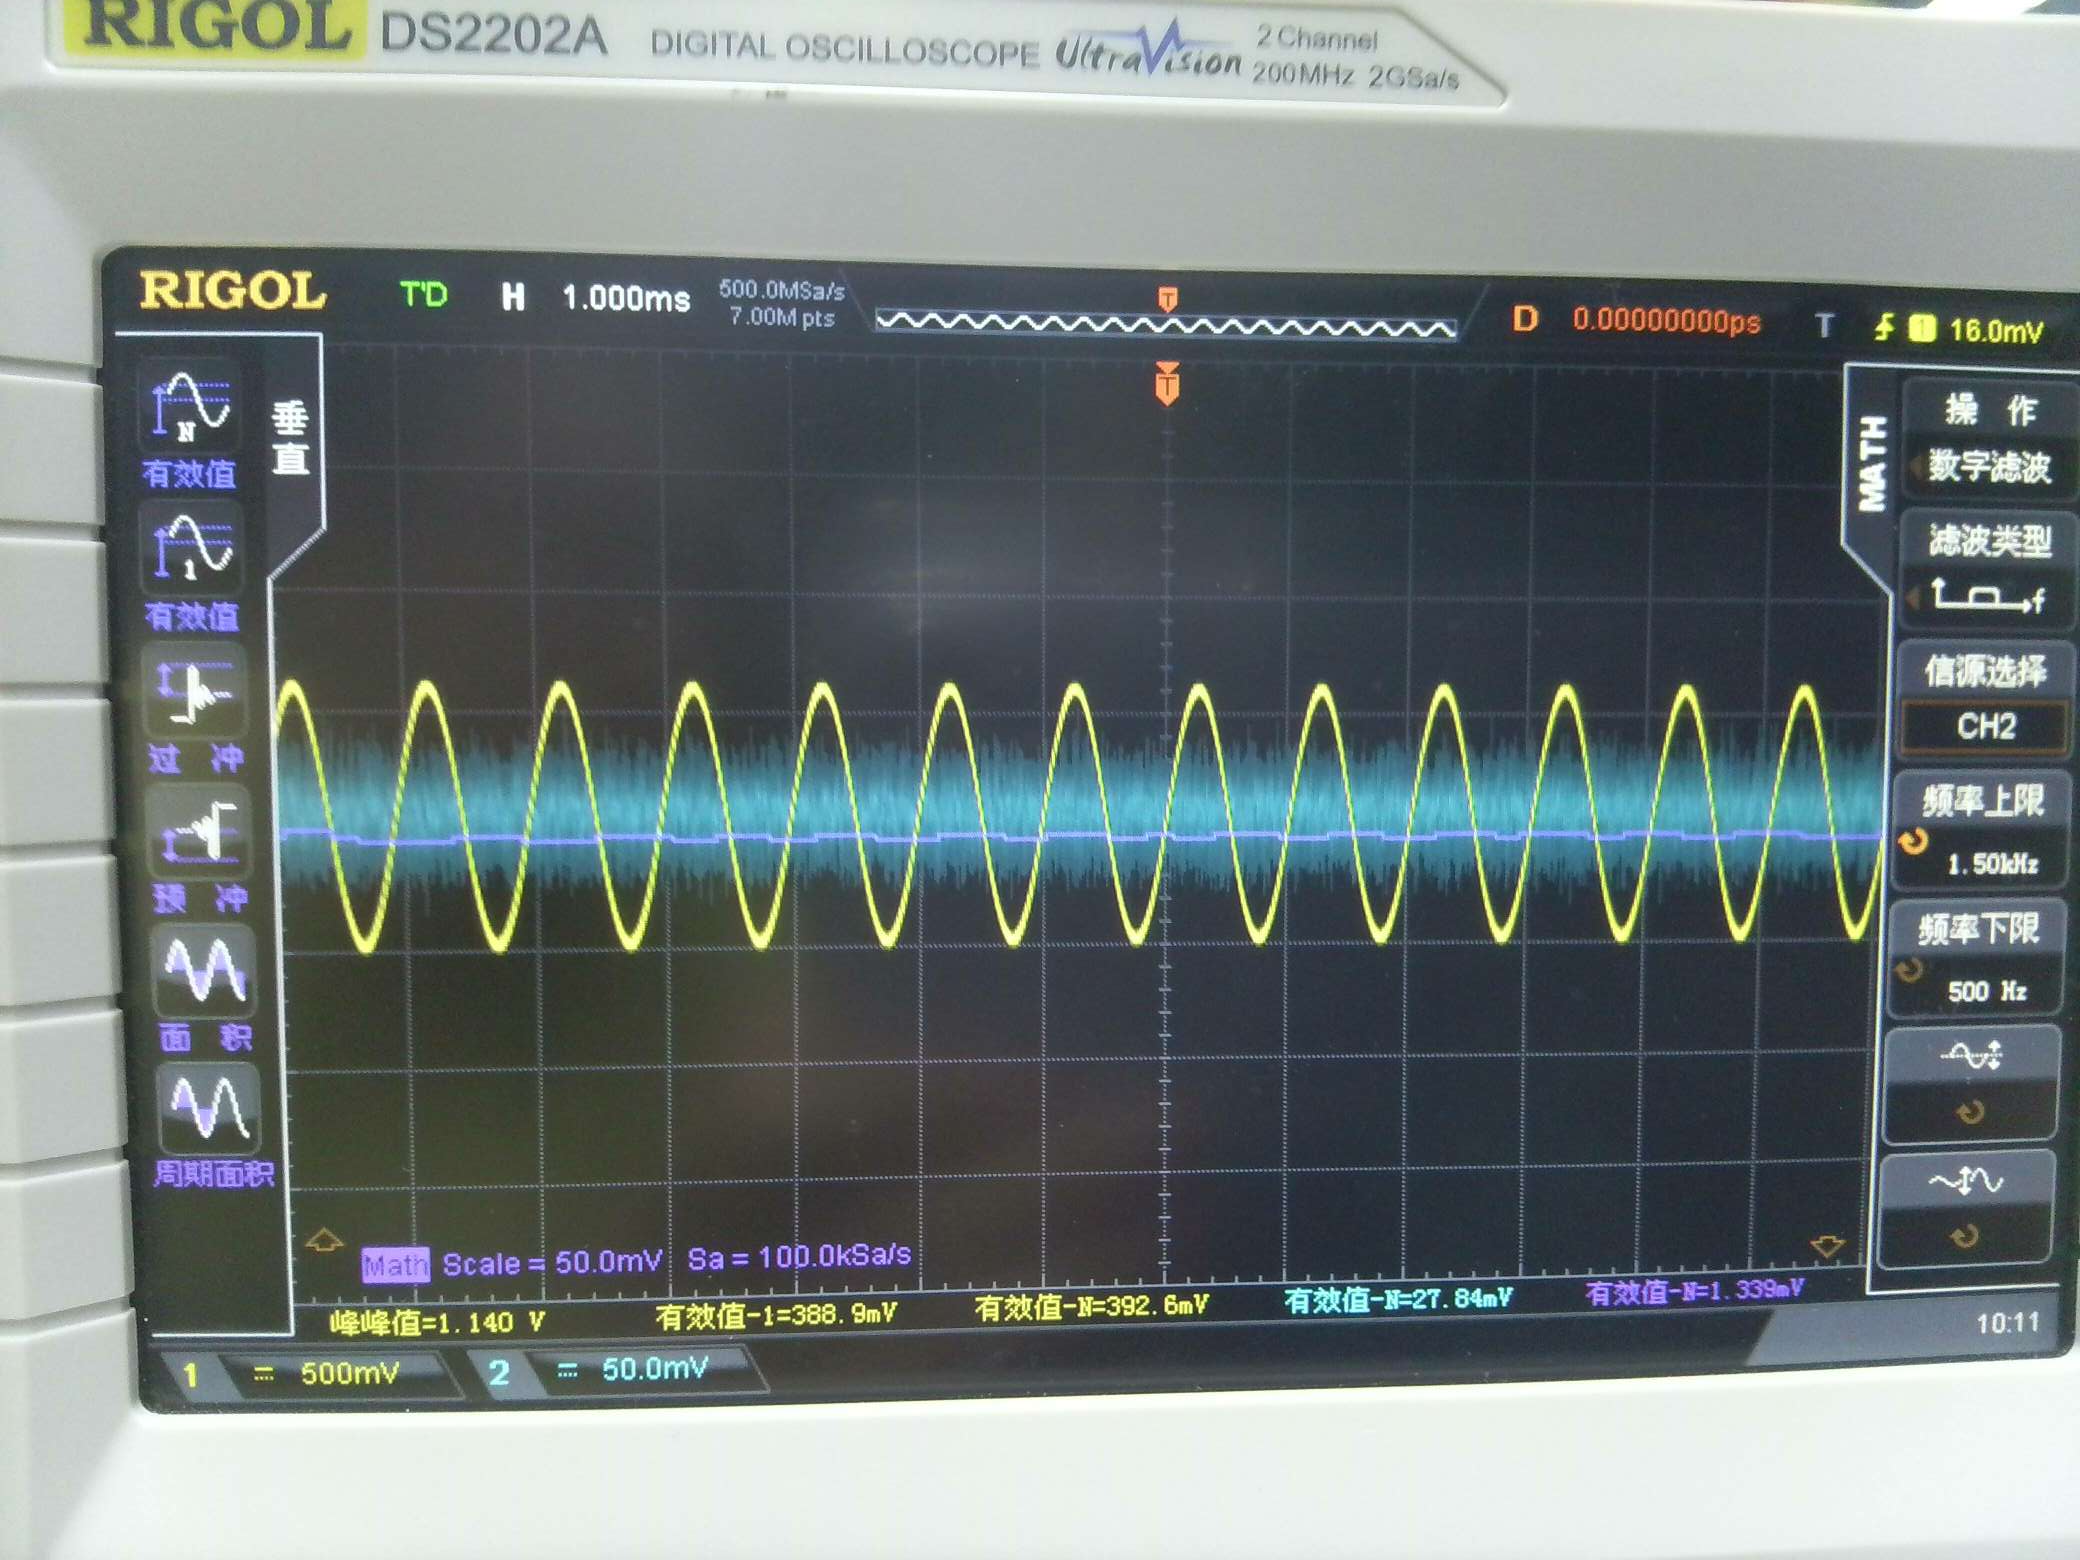
\includegraphics[width=3cm]{待测信号V_in波形图2.png}&\includegraphics[width=3cm]{待测信号V_in波形图3.png}\\
					\hline
					% 第六行
					& 滤波器带宽(Hz)&1.50k-500=1k & 1.50k-500=1k &1.50k-500=1k  \\
					\hline
					% 第七行
					& 滤波后信号有效值(m$V_rms$)&44.3 & 无 &无  \\
					\hline
					% 第八行
					& $SNR_{o,os}$(dB)&1.2868 & 无 &无  \\
					\hline
					% 第一行
					锁相放大器& 量程灵敏度(mV)&100& 200uV &10mV  \\
					\hline
					% 第二行
					&时间常数(mS)&1S& 3S &3S \\
					\hline
					% 第三行
					&陡降(dB/oct)&24&24 &24\\
					\hline
					% 第四行
					% 第五行
					&$V_{s,rms}$$mV_{rms}$&38.2& 38.33uV&3.82uV\\
					\hline
					% 第六行
					&R$mV_{rms}$&0.02& 38.3-41.2到 39.8uV&4.1-6.5到5.3mV\\
					\hline
					% 第七行
					&$SNR_{o,lo}$(dB)&65.6&11.1&0.339\\
					\hline
					% 第八行
					&信号发生器设定$mV_{rms}$&38.3&383&38.3\\
					\hline	
				\end{tabularx}
			\caption{强噪声背景下的弱信号检测实验记录}
			\label{tab:强噪声背景下的弱信号检测}
		\end{table}

\subsection{实验原始数据记录}
	\begin{figure}[htbp]
			\centering
			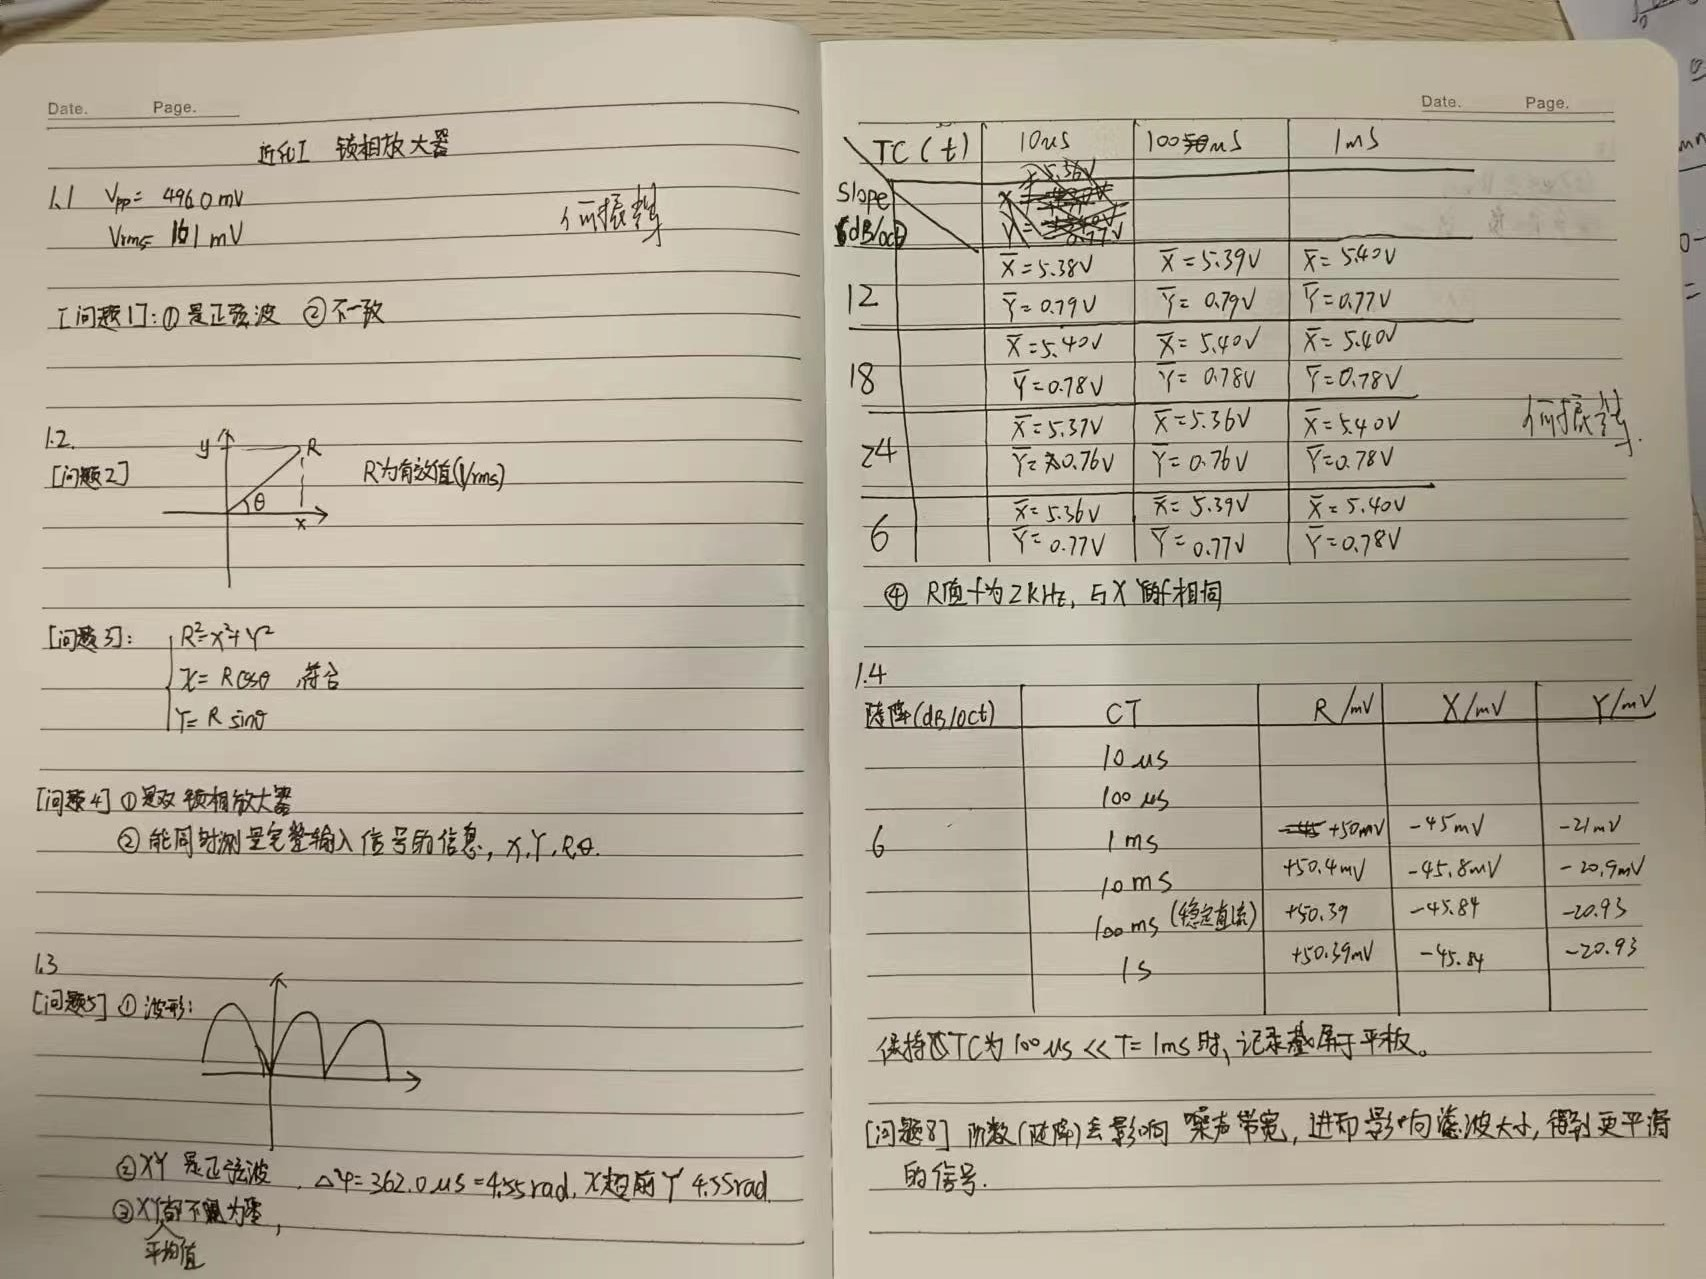
\includegraphics[width=0.75\textwidth]{实验原始数据记录.jpg}
			\caption{实验原始数据记录}
			\label{fig:实验原始数据记录}
	\end{figure}

	\clearpage
\begin{table}
	\renewcommand\arraystretch{1.7}
	\begin{tabularx}{\textwidth}{|X|X|X|X|}
	\hline
	专业:& 物理学 &年级:& 2022级\\
	\hline
	姓名: &丁侯凯 & 学号:&22344009 \\
	\hline
    日期:&2024.9.18 & 评分: &\\
	\hline
	\end{tabularx}
\end{table}

\nsection{D1}{锁相放大器与弱信号测量}{分析与讨论}
\subsection{实验数据分析}
	实验1.1 \quad  用示波器观察内部信号输出(与参考信号同频同相)

	\textbf{【问题一】示波器是否显示出正弦波?其测量的信号参数值是否与锁相放大器的信号设置值一致?}

	由图\ref{fig:示波器正弦波}可得,示波器显示为正弦波,测量的有效值为85.53mV,与锁相放大器的设定值$V_{set}=80mV$一致,并且测量得到的频率f=1.000kHz,也与设定值一致。

	实验1.2 \quad  用示波器观察内部信号输出(与参考信号同频同相)

	\textbf{【问题二】请比较示波器的读数和锁相放大器的R值,以理解R值的确切含义。}

	由图\ref{fig:示波器正弦波}可得,锁相放大器的测量R=81.4mV,与示波器测量的有效值相近,说明锁相放大器测量的R值为信号的有效值。

	\textbf{【问题三】测量数据反映出R、X、Y与$\theta$之间是什么关系?是否与式(D1-21)、(D1-24)和(D1-25)符合?}

	由实验测量数据可得:
	$$
	Rcos\theta=81.43mV *cos(177.33°) = -81.342mV \approx X
	$$
	$$
	Rsin\theta=81.43mV *sin(177.33°) = 3.79mV  
	$$
	$$
	Y\sqrt{X^2 + Y^2} =81.43mV \approx R
	$$
	计算说明,R、X、Y与$\theta$之间的关系符合式(D1-21)、(D1-24)和(D1-25)。

	\textbf{【问题四】你使用的OE1022是双锁相放大器吗?为什么?}

	是双锁相放大器,因为通过实验,发现可以同时测量完整的输入信号的信息,包括有效值R、相位角$\theta$与频率。

	实验1.3 \quad   相敏检波器工作原理——乘法器

	\textbf{【问题五】示波器上看到的什么波形?X、Y是正弦波吗?其相位差是多少度?X、Y的平均值为0吗?平均值是否会随着滤波器参数而改变?参照式(D1-19)和(D1-23)讨论:R值是否会呈现全波整流的正弦信号,其频率为多少?与X或者Y的频率存在什么关系?对比式(D1-28)讨论。}

	根据\ref{tab:1}可得,X、Y并不是纯正的正弦波,而是正弦波加上一个直流偏置,并且两者之间的相位差恒定为90°。经过D1-19得,$cos\theta$为直流项。

	由\ref{tab:2}可得增大时间常数,会改变滤波器参数,因为有高频分量的存在,所以波形的平均值并不为零。并且滤波器的参数会影响滤波效果,带宽越窄,滤波器对高频分量的抑制效果越好,输出波形的平均值越接近纯粹的直流分量。

	由\ref{eq:2}可得,输出的双倍频率正弦波类似于全波整流信号,因为公式中有输入信号的两倍和二次谐波成分,所以与输入信号相比,其频率加倍,但R与X、Y的波形的频率依旧相同。

	实验1.4 \quad   相敏检波器工作原理——乘法器+低通滤波器

	\textbf{【问题六】当调大时间常数后,输出R是否越来越稳定?直流分量(信号平均值)是否有所改变?}

	增加时间常数后,锁相放大器的低通滤波器的带宽降低,这有助于更有效地过滤掉高频噪声和不需要的频率成分,使得R信号中的高频部分被滤除。因此,时间常数增加,信号的平均值变得更加稳定。

	\textbf{【问题 7】 观察示波器波形,并给出在某一陡降值下,时间常数为多少个信号周期时,才能观察到稳定的直流输出?提示:注意调节示波器$Y$轴量程以提高测量振幅变化的精度。并结合式(D1-32)讨论。}

	式(D1-32)为
		\[
			R(t) = \frac{s(t)}{[1 + (\Delta\omega R C)^2]^{\frac{n}{2}}}
		\]

		由此可得:

		\begin{enumerate}
			\item 滤波器对输入信号的影响主要体现在分母部分。当输入信号的频率与参考信号频率不一致时,存在频率偏差 \( \Delta\omega \),此时信号 \( R(t) \) 会随着频率偏差的增加而逐渐衰减。
			
			\[
			\text{若} \Delta\omega = 0 \text{,则} R(t) = s(t) \text{,即信号未受影响。}
			\]
			
			\[
			\text{若} \Delta\omega \neq 0 \text{,滤波器将开始对信号进行衰减,偏差越大,衰减越明显。}
			\]
			
			因此,时间常数 \( \tau = RC \) 越大,滤波器的带宽越窄,可以更有效地滤除与参考频率不匹配的信号成分,提升信号的稳定性。
			
			\item 滤波器阶数 \( n \) 的影响:
			
			滤波器的阶数 \( n \) 决定了信号幅度随频率偏差 \( \Delta\omega \) 的衰减速率。
			
			\[
			\text{对于低阶滤波器:} n = 1 \text{(6 dB/oct),信号衰减较慢,允许较大的频率偏差。}
			\]
			
			\[
			\text{对于高阶滤波器:} n = 4 \text{(24 dB/oct),信号衰减更快,频率稍有偏差时,信号就会明显衰减。}
			\]
			
			高阶滤波器能够更好地滤除噪声,使信号更加稳定。
			
			\item 时间常数与信号稳定性之间的关系:
			
			随着时间常数 \( \tau = RC \) 的增大,公式中的项 \( (\Delta\omega R C)^2 \) 也增大,滤波器可以更加有效地抑制偏离中心频率的信号成分,使 \( R(t) \) 更加稳定。
			
			\item 信噪比的影响:
			
			通过调节滤波器带宽(即时间常数 \( RC \)),可以有效提高信号的信噪比。带宽越窄,滤波器允许通过的频率范围越小,从而可以滤除更多的噪声。时间常数越大,带宽越窄,信噪比提高,信号更加稳定。
			
		\end{enumerate}


		\textbf{【问题 8】为何在 1 阶(6dB/oct)时还没怎么起滤波效果,而到 4 阶(24dB/oct)时,则可看见明显的效果?}
		
		因为陡降表示信号在截止频率处的衰减速度,滤波器的阶数越高,陡降越陡,能更有效地去除高频噪声。所以,陡降越陡,滤波器在其截止频率附近的频率选择性就越好,即滤波效果越明显。
		并且由\ref{tab:2}可得:陡降设置的越大,输出波形的幅值越小,滤波效果越明显。

	实验1.8 \quad 强噪声背景下的弱信号检测

	\textbf{【问题 12】如何获得幅值为 0.1mVrms 的正弦波输入信号?}

可以考虑通过噪声发生器的信号端接口的 -80dB 衰减开关来解决。首先生成一个较大的信号,再经过衰减后得到所需的信号。如下所示:
\[
- 80 \, \mathrm{dB} = 20 \log \frac{V_{\text{out}}}{V_{\text{in}}} = 20 \log \frac{0.1 \, \mathrm{mVrms}}{V_{\text{in}}}
\]

根据公式,可以计算出输入信号的幅值:
\[
\Rightarrow V_{\text{in}} = 10000 \times 0.1 \, \mathrm{mVrms} = 1 \, \mathrm{Vrms}
\]

因此,可以使用信号发生器产生一个 1 Vrms 的正弦波信号,并通过噪声发生器的信号端接口的 -80dB 衰减开关,获得幅值为 0.1mVrms 的正弦波输入信号。

\textbf{【问题 13】对低信噪比信号或非周期噪声测量,能否用示波器的“auto”键?若通过手动调节,示波器屏宽(时间轴范围)应为多少个信号周期为宜?}

不能用auto进行调节,因为“auto”模式会首先检测输入信号的特征,包括频率、幅度和波形类型,根据信号的周期性,示波器会自动选择合适的时间轴范围,以确保信号在屏幕上完整显示,而本实验中是非周期信号,无法使用该模式。

用手动调节时,应该将图像缩小至连成粗线,这样可一个保证采样点足够概括大部分非周期点,防止周期过少导致信号不稳定。

\textbf{【问题 14】在用示波器观察、测量信号有效值时,请注意屏幕时间轴范围应达到待观测信号完整周期的整数倍;为什么?
}
由式子
\[
			u_{rms} = \frac{\int_0^{t} (u(\tau))^2 \mathrm{d\tau}}{t} \approx \frac{\int_0^{nT} (u(\tau))^2 \mathrm{d\tau}}{nT} = \frac{n\int_0^{T} (u(\tau))^2 \mathrm{d\tau}}{nT} = \frac{\int_0^{T} (u(\tau))^2 \mathrm{d\tau}}{T}
		\]
		可得:信号有效值的计算基于信号的平方在时间上的平均,且“$\approx$”仅在“积分时间$t$远大于周期$T$”,或“积分时间$t$是周期$T$的整数倍”时才成立,因此屏幕时间轴范围应达到待观测信号完整周期的整数倍。

\textbf{【问题 15】用锁相放大器测量 $R$ 值时,读数应保留几位有效数字?调节锁相放大器的什么参数设置可以得到?调节锁相放大器的什么参数可以获得稳定的读数。}

通过设置合适的时间常数和陡降,可以获得稳定的读数,应在取得2-3位稳定示数后,保留2-3位有效数字。或者设置合适Sensitivity,可以使得有效数字位数显示的尽可能多且保证一定的测量精度。


\subsection{实验报告思考题}
	\begin{question}
		描述用教学实验箱配制不同信噪比信号的原理;实验箱生成的噪声是否为白噪声?
	\end{question}
		1.信噪比信号配制的原理:

		通过将目标信号与噪声信号按一定比例叠加,从而控制信号的强度与噪声强度的相对大小。信噪比是信号功率与噪声功率的比值,通常以分贝(dB)为单位表示。
        
		通过实验箱内部通常具备波形发生器,可以生成所需的信号;
		通过内部噪声发生器生成噪声,常见的是白噪声,功率在所有频率均匀分布,或其他类型的噪声,如粉红噪声。
		随后通过实验箱的信号处理模块,将信号和噪声按不同的比例叠加。改变噪声的幅度或信号的幅度即可改变信噪比。
		
		信噪比可表示为:
		\[
		\text{SNR (dB)} = 10 \cdot \log_{10} \left(\frac{P_{\text{signal}}}{P_{\text{noise}}}\right)
		\]
		其中,\( P_{\text{signal}} \) 是信号的功率,\( P_{\text{noise}} \) 是噪声的功率。

		2. 实验箱生成的噪声是否为白噪声?

		白噪声的特点是它的功率谱在所有频率范围内是均匀分布的,即各个频率的噪声分量都是等量的。它在许多实验中用于模拟真实的背景噪声或干扰,因为它具有简单的统计特性,并且在时域上是随机的。

		


	\begin{question}
		随着信噪比的改变,信号R和相位差的测量值会有什么影响?
	\end{question}
	随着信噪比(SNR)的改变,信号幅度 \( R \) 和相位差 \( \theta \) 的测量值将受到显著影响。信噪比越高,信号的检测精度越高,噪声干扰越小;相反,随着信噪比的降低,噪声的影响增大,导致测量结果不准确或波动增大。

	1.信号幅度 \( R \) 的影响
	
	当信噪比较高时,噪声成分较少,信号幅度 \( R \) 的测量结果接近真实值。信号在较大噪声背景下能被清晰分离,测量结果稳定
	;当信噪比较低时,噪声占主导地位,信号幅度 \( R \) 可能被噪声掩盖,导致测量结果不准确,可能出现过度估计或低估信号幅度的情况。

	 2. 相位差 \( \theta \) 的影响
	在较高信噪比下,信号的相位差测量通常较为准确,因为信号的相位特征不会被噪声干扰破坏;在低信噪比条件下,噪声可能会显著影响相位测量,导致相位不稳定或出现大的测量误差。特别是在相位差较小的情况下,噪声的随机性可能导致相位测量发生较大的偏差。
	
	在锁相放大器等高精度测量仪器中,信噪比的降低会导致信号与参考信号之间的相位差测量变得困难,因为信号的相位在噪声的干扰下容易产生随机波动。信号的幅度测量也会因为噪声的叠加而产生随机误差,尤其是在信号强度较弱、噪声较强的情况下。

	因此,信噪比对信号的 幅度 \( R \)和 相位差 \( \theta \)的测量都有显著影响。提高信噪比有助于获得更精确的测量结果,而降低信噪比会增加测量误差。

	\begin{question}
		所有的噪声都可以用锁相放大器消除吗?锁相放大器的理论检测极限是多少?受什么限制?
	\end{question}
	1. 是否所有噪声都能通过锁相放大器消除?

	并非所有噪声都能通过锁相放大器消除。

	锁相放大器(LIA)擅长消除与信号频率无关的宽带噪声或随机噪声,例如热噪声、电子器件的本底噪声等。LIA通过对输入信号与参考信号进行相位同步,提取出特定频率范围内的信号,从而有效地抑制其他频率成分的噪声。

	然而,锁相放大器的噪声消除效果取决于噪声的频率特性:
	锁相放大器的可以消除有效消除宽带噪声(如白噪声)、随机噪声。

	锁相放大器难以消除的噪声:1)相位噪声:与信号频率相近的相位噪声可能影响LIA的性能,特别是当相位噪声与信号频率接近或相同,LIA很难将它们区分开。
	
	2)共频噪声:当噪声与信号处于相同频率或具有相位相关性时,LIA无法有效区分出信号和噪声。这类噪声可能是工频噪声(如50Hz或60Hz的电源干扰),若频率与信号频率相同,将直接影响测量。

	2. 锁相放大器的理论检测极限

	锁相放大器的理论检测极限受限于信号噪声比(SNR)。它的性能通常以最小可检测信号或信号分辨率来衡量。理论上,LIA可以检测到非常微弱的信号,但受到的限制因素有:噪声水平、时间常数和滤波器
	锁相放大器中的时间常数、参考信号的稳定性、环境干扰

	\begin{question}
		请比较锁相放大器与示波器(经过带通滤波后)测量不同信噪比信号的结果,分析两种测量仪器(方法)的优势与劣势。选择锁相放大器窄带宽的LPF可以降低式(D1- 33)中的$n _{\omega_r}$,从而提高测量值的信噪比吗?信噪比的提高与LPF带宽有何关系?参考式(D1-10)讨论。
	\end{question}
	锁相放大器与示波器(经过带通滤波后)测量不同信噪比信号的优劣:

	1. 锁相放大器(LIA):
	
	优点:

	1)窄带检测:
	
	锁相放大器能够在特定频率范围内对信号进行窄带滤波,并抑制其他频段的噪声。这使得它特别适用于在强噪声环境下检测微弱信号。

	高信噪比(SNR):由于锁相放大器的相敏检测原理,它可以显著提高信噪比,特别是在信号与噪声频率不同的情况下,能够通过锁定频率有效去除带外噪声。

	相位测量:锁相放大器能够精确地测量信号的相位信息,尤其是在测量频率相对稳定的信号时,这对相位相关的测量非常重要。
	
	缺点:

	1)响应速度较慢:
	
	由于低通滤波器的作用,锁相放大器在提高信噪比的同时降低了系统的响应速度,适合测量慢变信号或稳态信号,而不适合快速动态变化的信号。
	适用范围有限:锁相放大器通常仅适用于特定频率范围,不能同时测量多个频率成分的信号。
	
	2. 示波器(带通滤波后):

	优点:

	1)广频带监测:
	示波器可以显示整个频谱范围的信号,能够同时观测多个频率成分。这使其非常适合分析复杂信号和瞬态信号。
	
	2)直观性强:示波器可以实时显示信号波形,直观展现信号的时域和频域特性,是调试电路和查看波形的理想工具。
	
	缺点:

	1)信噪比有限:即使示波器配有带通滤波器,它的信噪比提升效果有限。由于示波器的滤波器带宽较宽,部分噪声仍然可能进入测量范围。
	
	2)缺少相敏检测:示波器通常不能直接测量信号的相位信息,这在某些应用中是一个劣势。

	\vspace{1cm}
	\textbf{选择锁相放大器窄带宽的LPF是否可以降低式(D1-33)中的 $n _{\omega_r}$,从而提高测量值的信噪比?}

	\begin{equation}
		R(t)= \sqrt{s^2(t) + n^2_{\omega_r} (t) + 2s(t)n _{\omega_r} sin(\omega_r + \theta)}
		\ne s(t)+ n_{\omega_r}(t)
		\label{eq:33}
	\end{equation}
其中:$R(t)$为放大器的输出的R值。
	
	选择锁相放大器中窄带宽的低通滤波器(LPF)可以降低式(D1-33)中的噪声功率 $n _{\omega_r}$,从而提高测量值的信噪比。
	
	在锁相放大器中,低通滤波器的带宽决定了通过滤波的噪声成分。噪声功率 $n _{\omega_r}$ 与滤波器带宽 \(B\) 成正比,经过LPF后,根据式(D1-33):
	

		信号的功率 \( P_{\text{signal}} \) 通常与滤波器带宽无关,因此总信噪比 \( \text{SNR} \) 可以表示为:
		
		\[
		\text{SNR} = \frac{P_{\text{signal}}}{P_{\text{noise}}} = \frac{P_{\text{signal}}}{N_0 \cdot B}
		\]
		
		从上式可以看出,信噪比与滤波器带宽 \( B \) 成反比关系。带宽越窄,噪声功率越小,从而信噪比越高;相反,带宽越宽,噪声功率越大,信噪比就会下降。

		如果以分贝(dB)为单位表示信噪比,则公式变为:

		\[
		\text{SNR(dB)} = 10 \cdot \log_{10}\left(\frac{P_{\text{signal}}}{N_0}\right) - 10 \cdot \log_{10}(B)
		\]
		
		这表明增加滤波器带宽 \( B \) 会降低信噪比; 减小带宽 \( B \) 则会提高信噪比,因为更多的噪声被滤除。因此,锁相放大器通过减小滤波器带宽可以有效地提高测量信号的信噪比,从而使得在低信噪比环境下也能对微弱信号进行准确测量。

	\vspace{1cm}
    \textbf{信噪比的提高与LPF带宽有何关系?参考式(D1-10)讨论。}
	D-10公式为:
\begin{equation}
	H(\omega) = \frac{1}{1+ J \omega R C}
	\label{eq:10}
\end{equation}
其中:$RC= \frac{1}{\omega_0}$表示时间常数,$\omega_0$为滤波器的截止频率。

信噪比与低通滤波器(LPF)带宽之间的关系可以通过滤波器的频率响应来分析。具体地说,低通滤波器的带宽决定了滤波后的噪声分量的大小,而噪声分量影响信号的信噪比。我们可以通过滤波器的传递函数 \( H(\omega) \) 和时间常数 \( RC \) 来进一步讨论这个问题。

考虑一个一阶低通滤波器,其传递函数为:

\begin{equation}
	H(\omega) = \frac{1}{1 + j\omega RC}
    \label{eq:6}
\end{equation}

其中:
 \( \omega \) 是信号的角频率。
 \( RC \) 是滤波器的时间常数,\( \omega_0 = \frac{1}{RC} \) 是滤波器的截止频率。

滤波器的带宽通常指滤波器允许信号通过的频率范围。在一阶RC低通滤波器中,带宽的大小主要由其截止频率 \( \omega_0 \) 决定,截止频率对应信号幅度衰减到其最大值的 \( 1/\sqrt{2} \)(约70%)的频率点。

根据信号与噪声的传输过程,滤波器会削弱高频噪声分量,但信号在通过低通滤波器时,频率低于 \( \omega_0 \) 的信号成分将基本保留,而频率高于 \( \omega_0 \) 的噪声将被削弱。因此,较窄的带宽 \( B \) 对降低噪声影响效果显著,从而提高信噪比。

由于噪声的总功率 \( P_{\text{noise}} \) 与滤波器带宽 \( B \) 成正比:

\[
P_{\text{noise}} \propto B
\]

而带宽 \( B \) 又与截止频率 \( \omega_0 \) 成正比,带宽越小,滤除的噪声越多,从而信噪比越高。因此,通过减小滤波器的截止频率 \( \omega_0 \) 或增大时间常数 \( RC \),可以有效减小噪声功率,进而提高信噪比。

结合传递函数公式 \ref{eq:6},我们可以看到,较大的 \( RC \) 值(对应较小的 \( \omega_0 \)):滤波器的截止频率变低,使得更多的高频噪声被滤除,因此信噪比提高;
较小的 \( RC \) 值(对应较大的 \( \omega_0 \)):滤波器的截止频率变高,带宽增大,更多的高频噪声通过滤波器,导致信噪比下降。

信噪比的提高与低通滤波器(LPF)带宽之间的关系是反比关系,带宽越窄,信噪比越高。通过调节滤波器的时间常数 \( RC \) 或截止频率 \( \omega_0 \),可以有效提高信噪比。在一阶低通滤波器中,较大的时间常数 \( RC \) 对应较窄的带宽,能够更好地抑制高频噪声,从而提高测量信号的信噪比。

\clearpage
% ---------------------------------------------------------------------
%   参考文献
%   注:使用参考文献时应按照xelatex->bibtex->xelatex->xelatex顺序进行编译
\phantomsection
\addcontentsline{toc}{section}{参考文献}
\bibliographystyle{unsrt} % 调整参考文献的格式,可供选择的有 plain, unsrt, alpha, abbrv, ieeetr, acm, siam, apalike 等。
\bibliography{myref}

% \clearpage
% \appendix
% \appendixpage
% \addappheadtotoc

% \begin{tbox}{字体设置(中文)}
% \begin{enumerate}
% 	\item 宋体:{\songti 山有扶苏,隰有荷华}
% 	\item 仿宋:{\fangsong 山有扶苏,隰有荷华}
% 	\item 黑体:{\heiti 山有扶苏,隰有荷华}
% 	\item 楷书:{\kaishu 山有扶苏,隰有荷华}
% \end{enumerate}
% \end{tbox}

% \begin{tbox}{Set font(English)}
% \begin{enumerate}
% 	\item roman:\quad{\rmfamily Hello world!}
% 	\item sans-serif:\quad{\sffamily Hello world!}
% 	\item typewriter:\quad{\ttfamily Hello world!}
% \end{enumerate}
% \end{tbox}

% \begin{tbox}{公式}
% 	无编号公式
%     \begin{equation*}
%         J(\theta) = \mathbb{E}_{\pi_\theta}[G_t] = \sum_{s\in\mathcal{S}} d^\pi (s)V^\pi(s)=\sum_{s\in\mathcal{S}} d^\pi(s)\sum_{a\in\mathcal{A}}\pi_\theta(a|s)Q^\pi(s,a)
%     \end{equation*}
% $$ J(\theta) = \mathbb{E}_{\pi_\theta}[G_t] = \sum_{s\in\mathcal{S}} d^\pi (s)V^\pi(s)=\sum_{s\in\mathcal{S}} d^\pi(s)\sum_{a\in\mathcal{A}}\pi_\theta(a|s)Q^\pi(s,a) $$
%     有编号公式
%     \begin{equation}
%         J(\theta) = \mathbb{E}_{\pi_\theta}[G_t] = \sum_{s\in\mathcal{S}} d^\pi (s)V^\pi(s)=\sum_{s\in\mathcal{S}} d^\pi(s)\sum_{a\in\mathcal{A}}\pi_\theta(a|s)Q^\pi(s,a)
%     \end{equation}
%     \begin{equation}
%         J(\theta) = \mathbb{E}_{\pi_\theta}[G_t] = \sum_{s\in\mathcal{S}} d^\pi (s)V^\pi(s)=\sum_{s\in\mathcal{S}} d^\pi(s)\sum_{a\in\mathcal{A}}\pi_\theta(a|s)Q^\pi(s,a)
%     \end{equation}
% 	波尔文积分
%     \[
%     \begin{cases}
%         \vspace{0.2cm}
%         \displaystyle{\int_{0}^{\infty} \frac{\sin(x)}{x}\dd{x} = \frac{\pi}{2}}\\
%         \vspace{0.2cm}
%         \displaystyle{\int_{0}^{\infty} \frac{\sin(x)}{x} \frac{\sin(x/3)}{x/3}\dd{x} = \frac{\pi}{2}} \\
%         \vspace{0.2cm}\cdot\cdot\cdot\\
%         \vspace{0.2cm}
%         \displaystyle{\int_{0}^{\infty} \frac{\sin(x)}{x} \frac{\sin(x/3)}{x/3} \cdot\cdot\cdot \frac{\sin(x/13)}{x/13}\dd{x} = \frac{\pi}{2}}\\
%         \displaystyle{\int_{0}^{\infty} \frac{\sin(x)}{x} \frac{\sin(x/3)}{x/3} \cdot\cdot\cdot \frac{\sin(x/15)}{x/15}\dd{x} = \frac{467807924713440738696537864469}{935615849440640907310521750000}\pi}
%     \end{cases}  
%     \]
% 	多行对齐公式
% 	\begin{align*} 
% 		\hat{H}^{(2)} &= \frac{1}{2}\sum_{\alpha}\sum_{\beta}\int \dd[3]{x}\dd[3]{x'} \hat{\psi}^\dagger_\alpha(\vb{x})\hat{\psi}_\beta^\dagger(\vb{x}')\qty[\sum_{\vb{q}\neq 0} \frac{4\pi e^2}{q^2}\mathrm{e}^{i\vb{q}\cdot(\vb{x}-\vb{x}')}]\hat{\psi}_{\beta}(\vb{x}')\hat{\psi}_\alpha(\vb{x})\\[.2cm]
% 		&=\frac{1}{2V}\sum_{\vb{k}}\sum_{\vb{k}'}\sum_{\vb{q}\neq 0}\sum_{\alpha}\sum_{\beta}\qty(\frac{4\pi e^2}{q^2})\hat{C}_{\vb{k}+\vb{q},\alpha}^\dagger\hat{C}_{\vb{k}'-\vb{q},\beta}^\dagger\hat{C}_{\vb{k}'\beta}\hat{C}_{\vb{k}\alpha}. 
% 	\end{align*}
% \end{tbox}

% \begin{tbox}{引用}
% 	对公式的引用,如\cref{equ:test}
% 	\begin{equation}
%         J(\theta) = \mathbb{E}_{\pi_\theta}[G_t] = \sum_{s\in\mathcal{S}} d^\pi (s)V^\pi(s)=\sum_{s\in\mathcal{S}} d^\pi(s)\sum_{a\in\mathcal{A}}\pi_\theta(a|s)Q^\pi(s,a)
% 		\label{equ:test}
%     \end{equation}
% 	对图像的引用,如\cref{fig:test}
% 	\begin{figure}[H]
% 		\centering
% 		
\includegraphics[width=0.3\textwidth]{example.png}
% 		\caption{测试图片}
% 		\label{fig:test}
% 	\end{figure}
% 	对表格的引用,如\cref{tab:test}
% 	\begin{table}[H]
% 		\renewcommand\arraystretch{1.5}
% 		\caption{一个空表格}
% 		\begin{tabularx}{\textwidth}{|p{0.15\textwidth}|X|X|X|X|}
% 		\hline
% 		 &  &  &  &  \\    
% 		\hline
% 		 &  &  & &  \\    
% 		\hline
% 		\end{tabularx}
% 		\label{tab:test}
% 	\end{table}
% \end{tbox}

% \begin{tbox}{表格}
% 	tabular可以自己更改宽度
% 	\begin{table}[H]
% 		\renewcommand\arraystretch{1.7}
% 		\centering
% 		\caption{一个空表格}
% 		\begin{tabular}{|p{0.15\textwidth}|p{0.15\textwidth}|p{0.15\textwidth}|p{0.15\textwidth}|}
% 		\hline
% 		&   &  &  \\
% 		\hline
% 		 &   &  &  \\
% 		\hline    
% 		\end{tabular}
% 	\end{table}
% 	tabularx可以自适应宽度
% 	\begin{table}[H]
% 		\renewcommand\arraystretch{1.7}
% 		\centering
% 		\caption{一个空表格}
% 		\begin{tabularx}{\textwidth}{|p{0.2\textwidth}|X|X|X|X|X|X|}
% 			\hline
% 			& &  &  &  &  &  \\
% 			\hline
% 			 & &  &  &  &  &  \\
% 			\hline
% 		\end{tabularx}
% 	\end{table}
% \end{tbox}

\end{document}
